\documentclass{article}
\usepackage{blindtext}
\usepackage[utf8]{inputenc}
\usepackage{fancyhdr}
\usepackage{amsmath}
\usepackage{amssymb}
\usepackage{amsthm}
\usepackage{tikz}
\usepackage{blkarray}
\usepackage{algorithm}
\usepackage{algpseudocode}
\usepackage{algorithmicx}
\usepackage{hyperref}
\usepackage{tikz}
\usepackage{pgfgantt}
\usepackage{listings}
\usepackage{xcolor}
\usepackage{wrapfig}
\usepackage{relsize}
\usepackage{eurosym}
\usepackage{parskip}
\usepackage{textcomp}
\usepackage{stackengine}
\usepackage{float}
\usepackage{bookmark}
\usepackage{caption}
\usepackage{forest}
\usepackage{mdframed}
\usepackage{cancel}
\usepackage{enumitem}
\usepackage{tabu}
\usepackage{tcolorbox}
\usepackage{multicol}
\tcbuselibrary{theorems,breakable}
\usepackage[a4paper, total={6in, 8in}]{geometry}
\usetikzlibrary{calc,trees,positioning,arrows,chains,shapes.geometric,decorations.pathreplacing,decorations.pathmorphing,shapes,matrix,shapes.symbols,fit,graphs,snakes}
\usepackage{nicefrac}


% Migliore grafica per i theorem/definition/properties/exercises/examples
\newtheoremstyle{break}% name
{2 \baselineskip}%         Space above, empty = `usual value'
{}%         Space below
{} %{\itshape}% Body font. I prefer empty body font
{\parindent}%         Indent amount (empty = no indent, \parindent = para indent)
{\bfseries}% Thm head font
{.}%        Punctuation after thm head
{\newline}% Space after thm head: \newline = linebreak
{}%         Thm head spec

\theoremstyle{break}

\newtcbtheorem[number within=section]{thm}{Teorema}%
{colback=green!5,colframe=green!35!black,fonttitle=\bfseries}{th}
\newcounter{def}
\newtcbtheorem[number within=section]{definition}{Definizione}%
{colback=red!5,colframe=red!35!black,fonttitle=\bfseries}{dfn}
\newcounter{prop}
\newtheorem{property}[prop]{Proprietà}
\newcounter{exer}
\newtheorem{exercise}[exer]{Esercizio}
\newcounter{exmp}
\newtcbtheorem[number within=section]{example}{Esempio}%
{breakable,colback=gray!5,colframe=gray!35!black,fonttitle=\bfseries}{exmp}
\newcounter{lmma}
\newtheorem{lemma}[lmma]{Lemma}
\tcolorboxenvironment{nota}{
blanker,breakable,left=5mm,
before skip=10pt,after skip=10pt,
borderline west={1mm}{0pt}{red}}

% TikzStyles
\tikzstyle{block} = [rectangle, draw, text centered]
\tikzstyle{empty_block} = [rectangle, text centered]
\tikzstyle{line} = [draw, -latex']
% /End TikzStyles

\definecolor{azzurro}{cmyk}{1,0.33,0,0.13}
\definecolor{arancione}{cmyk}{0,0.41,1,0}
\definecolor{verde}{cmyk}{0.44,0,0.38,0.31}
\definecolor{viola}{rgb}{0.58,0,0.82}
\definecolor{bianco}{rgb}{0.95, 0.95, 0.92}
% C style
\lstdefinestyle{CStyle}{
    backgroundcolor=\color{bianco},   
    commentstyle=\color{verde},
    keywordstyle=\color{viola},
    numberstyle=\tiny\color{arancione},
    stringstyle=\color{azzurro},
    basicstyle=\footnotesize,
    breakatwhitespace=false,         
    breaklines=true,                 
    captionpos=b,                    
    keepspaces=true,                 
    numbers=left,                    
    numbersep=5pt,                  
    showspaces=false,                
    showstringspaces=false,
    showtabs=false,                  
    tabsize=2,
    language=C
}
\lstset{
  basicstyle=\ttfamily,
  columns=fullflexible,
  frame=single,
  breaklines=true,
  postbreak=\mbox{\textcolor{red}{\(\hookrightarrow\)}\space},
}
% maximum matrix environment set to 50 instead of 10
\setcounter{MaxMatrixCols}{50}

\newcommand{\norm}[1]{\left\lVert#1\right\rVert}
\newcommand{\abs}[1]{\left|#1\right|}
\newcommand{\R}{\mathbb{R}}
\newcommand*\circled[1]{\tikz[baseline= (char.base)]{
            \node[shape=circle,draw,inner sep=2pt] (char) {#1};}}
\newcommand{\coloredbox}[1]{\fcolorbox{black}{#1}{\rule{0pt}{6pt}\rule{6pt}{0pt}}\quad}

% Text under-above matrix https://tex.stackexchange.com/a/78467
\newenvironment{spmatrix}[1]
  {\def\mysubscript{#1}\mathop\bgroup\begin{pmatrix}}
  {\end{pmatrix}\egroup_{\textstyle\mathstrut\mysubscript}}

\newenvironment{sbmatrix}[1]
  {\def\mysubscript{#1}\mathop\bgroup\begin{bmatrix}}
  {\end{bmatrix}\egroup_{\textstyle\mathstrut\mysubscript}}

% per le nostre cagate
\newcommand{\checkeditem}{\item[\refstepcounter{enumi}$\text{\rlap{$\checkmark$}}\square$]}
\newlist{todolist}{itemize}{2}
\setlist[todolist]{label=$\square$}

% Euro workaround - https://tex.stackexchange.com/questions/110972/eurosym-seems-to-not-be-working
\DeclareRobustCommand{\officialeuro}{%
  \ifmmode\expandafter\text\fi
  {\fontencoding{U}\fontfamily{eurosym}\selectfont e}}

% forest
\forestset{
  every leaf node/.style={
    if n children=0{#1}{}
  },
  every tree node/.style={
    if n children=0{}{#1}
  },
  edgelabel/.style n args={2}{
    edge label={node[midway,#1]{#2}}
  },
  nodevalue/.style n args={2}{
    label=#1:{{#2}}
  }
}
\forestset{
  suffix tree/.style={
    for tree={
      edge={->},
      every tree node={
        circle, draw, minimum size=1.5em, s sep=1cm,
        s sep+=1em,
        l sep+=1em
      },
      every leaf node={
        rectangle, draw, 
        minimum size=1.5em
      }
    }
  }
}
\forestset{
  highlight ancestors/.style={
    before typesetting nodes={
      for current and ancestors=highlight
    }
  },
  highlight/.style={
    draw=darkgray,
    edge+=red
  }
}
\forestset{
  terminal/.style={
    if n children=0{
    tier=terminal
    }{}
  }
}
\usepackage{parskip}

\title{Analisi e Progettazione Algoritmi}
\author{Adrian Castro, Ilaria Battiston \thanks{Slides di Mauri}}
\date{Ottobre 2018}
\pagestyle{fancy}

\begin{document}

\maketitle

\lfoot{}
\cfoot{}
\rfoot{\thepage}

\newpage
\tableofcontents
\newpage
\section{Introduzione}

\subsection{Chiarimenti sul corso}

\begin{enumerate}
    \item Ricevimento U14 1010 1$^\circ$ piano;
    \item \href{mailto:zandron@disco.unimib.it}{zandron@disco.unimib.it};
    \item Modalità d'esame: \begin{enumerate}
        \item Scritto: esercizi + teoria;
        \item Verbalizzazione normale;
        \item Compitini: \begin{enumerate}
            \item 1o: esercizi;
            \item 2o: esercizi + teoria.
        \end{enumerate}
    \end{enumerate}
\end{enumerate}

\subsection{A grandi linee}

\subsubsection{Programmazione dinamica}
La programmazione dinamica è un metodo di risoluzione dei problemi che consiste nel trovare sotto-informazioni che poi verranno riutilizzate con il tempo. Il problema viene spezzato in parti, e si cerca di trovare una sotto-informazione che può essere sfruttata quando necessario. Efficiente in termini di spazio e tempo. 

Alcuni algoritmi hanno una soluzione intuitiva, ma che richiedono di ricalcolare tante volte la stessa cosa. Una soluzione può essere usare una \textbf{cache}, memoria dove vengono salvati i valori calcolati precedentemente. A questo punto, però, l'algoritmo è meno efficiente dal punto di vista dello \textbf{spazio}. Bisogna quindi capire in quali casi è opportuno attuare una tecnica del genere. 

La programmazione dinamica viene usata nei problemi di ottimizzazione e di decisione. Gli algoritmi di decisione devono saper rispondere a ogni tipo di input (es. esiste un cammino che collega due nodi?). 

Un altro problema è la ricerca: dato un input $x$, determinare una soluzione $S$ che rispetti le caratteristiche del problema. Deve esistere $S$ tale che esista un collegamento $(x,\ S)$. 

L'ottimizzazione associa a ogni soluzione il relativo costo e cerca la miglior soluzione possibile in base al costo minimo: $S^*\:|\:C(S^*) \leq C(S)$. \\
Bisogna considerare anche che alcune soluzioni non sono ammissibili.

\subsubsection{Programmazione reedy}
Il tipo di programmazione \textbf{greedy} (o \textbf{goloso}), viene usata per determinare la soluzione migliore tramite una serie di calcoli effettuati localmente, per esempio previsioni in base ai dati correnti. Non si conosce l'andamento dei dati nel futuro. \par
Una tecnica di programmazione \textbf{greedy} si basa sulla situazione attuale per capire cosa fare successivamente. \par
Esempio: problema del $travelling\ salesman$. La tecnica greedy continua a ridurre le possibilità di scelta, più avanti si va nell'algoritmo. Ciò significa che le scelte attuali di viaggio possono sembrare poco costose, ma poi magari ci si ritrova con le ultime scelte che hanno spese insostenibili. \par
In casi di questo tipo, un algoritmo \textbf{greedy} non è la scelta più adatta. Possiamo quindi fare la seguente osservazione:
\begin{definition}{Algoritmo Greedy}{greedy}
    Gli algoritmi di tipo greedy funzionano al meglio se tutti i pesi (o valori) delle scelte sono uguali a $1$.
\end{definition}
$$
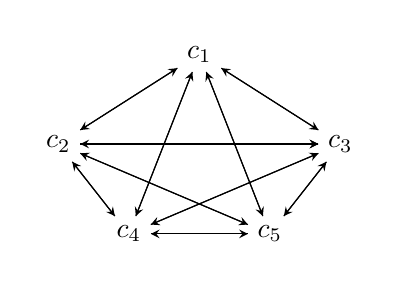
\begin{tikzpicture}
    \matrix (m) [matrix of math nodes, row sep=2em,
    column sep=1em]{
    & & c_1 & & \\
    c_2 & & & & c_3 \\
    & c_4 & & c_5 & \\};
    \path[-stealth]
    (m-1-3) edge (m-2-1) % c1
            edge (m-2-5)
            edge (m-3-2)
            edge (m-3-4)
    (m-2-1) edge (m-2-5) % c2
            edge (m-2-5)
            edge (m-3-2)
            edge (m-1-3)
            edge (m-3-4)
    (m-2-5) edge (m-2-1) % c3
            edge (m-1-3)
            edge (m-3-4)
            edge (m-3-2)
    (m-3-2) edge (m-1-3) % c4
            edge (m-2-1)
            edge (m-2-5)
            edge (m-3-4)
    (m-3-4) edge (m-1-3) % c5
            edge (m-2-1)
            edge (m-2-5)
            edge (m-3-2);
\end{tikzpicture}
$$

Alcuni algoritmi sui grafi implementabili con uno dei due metodi di programmazione sono BFS, DFS, cammini minimi, problemi di flusso.
Quando nessun algoritmo è in grado di risolvere un problema in tempo accettabile (non esponenziale) si parla di NP-completezza.
\section{Introduzione}
I database non consistono solo in dati e tabelle: sono modelli centralizzati o distribuiti che permettono di gestire un carico anche significativo di utenti. La sicurezza è un aspetto importante, insieme all'affidabilità: i sistemi relazionali hanno grandi utilizzi nei settori bancari, e le operazioni devono giungere a termine senza guasti.

I DBMS sono quindi sistemi che devono garantire la gestione di dati di grandi dimensioni, persistenti, affidabili e condivisi. Oltre ai modelli relazionali esistono i NoSQL (Not Only SQL) e RDF, i quali hanno vantaggi e svantaggi a seconda dell'utilizzo.

Per garantire le precedenti caratteristiche, l'architettura di un DBMS deve avere una serie di funzionalità cooperanti, come un gestore delle transazioni, un query compiler e un gestore della memoria secondaria.

\section{Strutture fisiche di accesso}
La più piccola struttura di memorizzazione dei dati a cui gli utenti possano accedere è il file: così come le tabelle, ha un'intestazione fissa e un numero di righe.

I dati non devono solo essere memorizzati in modo persistente: devono anche essere facilmente recuperabili, e gli accessi da gestire sono sia in lettura che in scrittura. Un obiettivo fondamentale è la minnimizzazione del tempo di accesso e trasferimento da CPU alla memoria secondaria.

I dati sono memorizzati nei dischi magnetici, con blocchi da 4-32kbyte e un tempo di accesso di circa $10^{-8}$ millisecondi, con un tasso di trasferimento di 300 Mbit/secondo. Il problema è la grande differenza di ordini di grandezza tra queste operazioni.

L'organizzazione ottimale è un compromesso tra il tempo e lo spazio, di cui il tempo è la priorità considerando il costo ridotto della memoria. 

\subsection{Campi in SQL}
Ogni campo in una tabella è memorizzato in una struttura fisica, ma lo spazio occupato cambia a seconda del tipo del dato. Le tuple sono pertanto record fisici organizzati in collezioni all'interno dei blocchi di memoria, e bisogna gestire anche modifica e cancellazione.

Esempi di tipi di dati:
\begin{itemize}
	\item VARCHAR, che alloca $n + 1$ bytes secondo un bit di carattere separatore o numero di caratteri;
	\item BLOB e GLOB, destinati a larghi file il cui spazio viene allocato solo al momento dell'inserimento.
\end{itemize}

I record possono avere formato e lunghezza fissi o variabili, con eventuali campi straordinari. Il record layout include informazioni supplementari con schemi o puntatori, lunghezza e timestamp di ultima lettura e scrittura. 

I record sono organizzati in blocchi, unità di memoria trasferite dal disco alla memoria principale. La dimensione è generalmente fissa a $2^n$, di cui solitamente alcuni byte non vengono utilizzati. 

Nel caso in cui la lunghezza sia variabile, lo header contiene anche la lunghezza del record e l'offset (distanza rispetto al byte iniziale) dei campi. I campi fissi sono allocati prima di quelli variabili. 

Alcuni record sono rappresentati in più blocchi, cioè spanned: anche questa informazione è contenuta nell'header, e l'ordinamento è gestito tramite la contiguità fisica o collegamento tra record (modello a grafo, sistemi scalabili). 

\subsection{Strutture di files}
I metodi di accesso sono algoritmi o moduli che forniscono primitive CRUD per ciascuna delle strutture.

Esempi di metodi di accesso sono: 
\begin{itemize}
	\item Strutture sequenziali;
	\item Strutture con accesso calcolato (hash);
	\item Strutture ad albero (indice).
\end{itemize}

L'accesso può essere sequenziale, binario o con indice. Il costo è determinato dallo spazio e dal tempo, ed è solitamente approssimato come il numero di blocchi acceduti. Per sceglere la struttura ottima è necessario distinguere se i file sono statici o dinamici e la frequenza delle operazioni CRUD.

\subsubsection{Sequenziali}
Le strutture sequenziali hanno in comune il mantenimento di un ordinamento fisico in memoria. Esistono organizzazioni per righe o per colonne.

\textbf{Non ordinata}: i nuovi record sono appesi in fondo al file nell'ordine in cui arrivano al DB, e l'ordine di visualizzazione è arbitrario. Il dato non è persistente finchè non viene scritto sul FS, quindi il blocco dev'essere copiato nel buffer e il record aggiunto. \\
La scansione è necessariamente sequenziale, quindi lettura e aggiornamento sono lente, e i record vengono periodicamente riorganizzata per sovrascrivere le cancellazioni.

\textbf{Ordinata}: la posizione fisica è determinata dal campo chiave, e l'ordinamento fisico è l'ordinamento delle chiavi. \\
La ricerca (anche per range) è semplice, ma la creazione impiega più tempo. La cancellazione dipende dallo schema di allocazione, ma richiede riorganizzazione periodica. 

Alcuni metodi per rimediare al tempo di inserimento sono l'append in coda con riordinamento periodico, (accesso logaritmico) oppure l'allocazione al posto di record cancellati. Può essere lasciato spazio libero per uso futuro, o possono esserci file di overflow con linked list.

\subsubsection{OLAP}
OLAP (On Line Analytical Processing) è la raccolta di dati il cui uso primario è per le decisioni organizzative. Un data warehouse è un carico di lavoro subject-oriented, integrato, non volatile e variabile con il tempo. 
	
Le informazioni sono rappresentate tramite un cubo dimensionale di cui gli assi indicano il tempo, i prodotti e i punti vendita. L'organizzazione è gerarchica, in categorie.

Non esiste un metodo generale per la modellazione di un DW: il modello ER dev'essere trasformato ed esteso, i dati devono essere permanenti e sono memorizzati in blocchi contenenti righe vicine tra loro. 

I dati sono salvati colonna per colonna per evitare scansioni multiple in query come COUNT, ma l'inserimento viene effettuato comunque con la riga (strutture row-oriented) che poi viene spostata.

\subsubsection{Hash}
Le tabelle hash permettono l'accesso diretto sulla base del campo chiave, in casi in cui una struttura ad array sarebbe inefficiente perché i possibili valori della chiave sono molti di più di quelli utilizzati.

I record sono organizzati in bucket (blocchi), e la funzione hash, generalmente il modulo, associa a ogni valore della chiave un indirizzo. Lo spazio delle chiavi è più grande dello spazio degli indirizzi (funzione non iniettiva) e ci sono possibilità di collisioni.

Le collisioni vengono gestite tramite tabella di overflow o extensible hashing. La tabella di overflow funziona come bucket aggiuntivo per gli hash duplicati, e l'eventuale spostamento con la cancellazione dei record.

Questo comporta la decisione della grandezza dei bucket e dei file: bisogna tenere in considerazione il numero medio di accessi. La probabilità di overflow cresce con il numero di record e decresce con la dimensione del blocco. 

Con $T$ records e $F$ record per bucket in media, il numero dei bucket $B$ dovrebbe essere $B = T / (0.8 \cdot F)$ per utilizzare il 50-80\% dello spazio disponibile.

Le strutture hash sono efficienti per accesso diretto con il valore della chiave, ma non funzionano per ricerche basate su range o campi diversi. La dimensione dei file non deve subire variazioni significative nel tempo.

L'extensible hashing consente la crescita indefinita della struttura ed elimina l'overflow: essa aumenta dinamicamente con accesso tramite directory, la quale definisce la funzione hash. 

Lo spreco di spazio è limitato, le riorganizzazioni sono solo a livello locale e il tempo di accesso è veloce. La directory va tenuta nella memoria principale.

\subsubsection{Strutture ad albero}
Le strutture ad albero (B-tree) si basano sull'utilizzo di un indice, una struttura ausiliaria per l'accesso efficiente ai record tramite un campo chiave (non necessariamente identificante).

Un indice è un altro file con record contenenti chiave e indirizzo, ordinato secondo i valori della chiave (indice analitico di un libro).







\section{Data analytics issues}

\subsection{Istanze, classi e attributi}
\textbf{Istanza} (oggetto, record): esempio descritto da un numero di attributi. \\
\textbf{Attributo} (campo, caratteristica): misura gli aspetti delle istanze. \\
\textbf{Classe}: gruppo di istanze.

Le istanze sono tipi specifici di esempi che devono essere classificati, associati ed eventualmente raggruppati. Possono essere \textit{dipendenti} o \textit{indipendenti} e sono caratterizzate da un numero predeterminato di attributi: l'input ai modelli di apprendimento sono istanze contenute in un dataset, basandosi su assunzioni \textbf{IID} (indipendenti e identicamente distribuite, derivano dalla stessa distribuzione).

La rappresentazione in forma proposizionale (tabellare) implica la definizione degli attributi, rimuovendo le relazioni ed esprimendole eventualmente tramite campi e condizioni. Viene considerato solo l'insieme delle osservazioni disponibili (``mondo chiuso"). 

Il processo di flattening di relazioni per creare un'unica tabella si indica con \textbf{proposizionalizzazione}: è possibile con qualsiasi insieme finito, ma causa ``biased models" con irregolarità o dati replicati rispetto al modello originale. Le relazioni $1 : n$ sono gestite associando un campo aggiuntivo nel lato 1 oppure con matrici booleane. L'operazione di \textit{join} generalmente causa rappresentazioni non totalmente veritiere (distorsioni), ma che hanno minore complessità computazionale.

Gli attributi sono le \textit{features} che costituiscono lo spazio di rappresentazione dell'input: devono sempre avere lunghezza predefinita, eventualmente si ricorre all'uso di flag. L'esistenza di alcuni attributi (derivabili) può dipendere da altri, e questo potrebbe aumentare la complessità del modello. 

Le variabili \textbf{nominali} (simboliche, categoriche, discrete) rappresentano una quantità nominale e non hanno relazioni logico-matematiche tra loro. \\
Le variabili \textbf{ordinali} (numeriche) impongono un ordine (numeri, stringhe). \\
Spesso non è immediata la distinzione tra nominali e ordinali. 

Conoscere la natura dell'attributo è essenziale per poter effettuare confronti e avere un criterio per le operazioni, trattare i dati mancanti e gestire le problematiche legate alla qualità dei dati.

\subsection{Data analytics tasks}
\subsubsection{Classification learning}
Supervisionato, si occupa della classificazione di campioni predefiniti in classi, secondo approcci di machine learning (regressioni, alberi di decisione, reti bayesiane). 

Il modello deve avere buone capacità di generalizzazione per input mai trattati prima, ed è possibile definire modelli di apprendimento in base a regole logiche su rappresentazioni proposizionali. Le regole logiche sono codificate usando \textit{if}.

\subsubsection{Clustering}
Il clustering serve per identificare gruppi di istanze simili. Gli algoritmi sono non supervisionati: la classe di un esempio non è conosciuta in partenza. Vengono utilizzati per la segmentazione.

\subsubsection{Associazione}
Modello predittivo non supervisionato con l'obiettivo della comprensione di associazioni: dall'esistenza di un attributo prevedere l'esistenza di un altro.

\subsubsection{Predizione numerica}
Supervisionato, modelli con un valore target in input: cerca di individuare relazioni tra attributi numerici (regressione).

\section{Data preprocessing}
I dati solitamente contengono problematiche che devono essere affrontate prima di poterli dare in input al modello: il preprocessing è un'attività fondamentale per individuare rumore, inconsistenze e incorrettezze.

Il processo di \textbf{data cleaning} si occupa di rimpiazzamento di valori mancanti e smoothing dei dati rumorosi. Ci sono modelli in grado di gestire per natura i missing values, ma altri hanno necessariamente bisogno della completezza. Non tutti i dati incompleti possono essere sostituiti.
\begin{itemize}
	\item MCAR (Missing Completely At Random): lla distribuzione di un esempio con valori mancanti non dipende da altri attributi;
	\item MAR (Missing At Random): la distribuzione di un esempio con valori mancanti dipende dagli attributi osservati, non necessariamente mancanti;
	\item NMAR (Not Missing At Random): la distribuzione di un esempio con valori mancanti dipende da attributi con valori mancanti.
\end{itemize}

I dati mancanti si possono ignorare, convertire a valori di default o rimpiazzare. Alcune tecniche di sostituzione implicano l'utilizzo della media (per valori continui con distribuzione normale) o della moda (discreti). Un altro modo è k-NN, che associa la classe sulla base della maggioranza degli oggetti vicini.

Un metodo di discretizzazione (smoothing) è il binning: divide il range in $N$ intervalli in base alla media (distribuzioni normali) o alla frequenza (skewed).



\section{Unbalanced data}
Una delle problematiche che riguardano modelli di apprendimento predittivi e prescrittivi si verifica quando la distribuzione dei campioni di una determinata classe sono molto più frequenti rispetto a un'altra (es. contesto medico). La maggior parte dei campioni sono corretti, ma inutili: non è necessario fare analisi sulla maggioranza, sapendone già il comportamento. 

Per bilanciare i dati si usano due tecniche:
\begin{itemize}
	\item Oversampling: costruzione di un dataset con un numero desiderato di campioni dalla classe di minoranza e uno uguale dalle altre;
	\item Undersampling: eliminazione di un numero arbitrario di campioni dalla classe di maggioranza, in modo da avere lo stesso numero rispetto alla classe di minoranza. 
\end{itemize}
Questi metodi sono applicabili con due classi, ma anche con un maggior numero. Ci sono algoritmi che si focalizzano su uno o sull'altro, e approcci ibridi che li combinano. Si assume che i dati siano corretti, rappresentativi e in assenza di rumore.

\subsection{SMOTE}
SMOTE (Synthetic Minority Oversampling Technique) è un algoritmo iterativo di oversampling:
\begin{enumerate}
	\item Per ogni campione di minoranza, trova i suoi $k$ elementi di minoranza più vicini;
	\item Di queste ne sceglie $n$ in modo casuale;
	\item Calcola il punto medio tra quello iniziale e ciascuno degli $n$ (Generated Synthetic Instance);
	\item Il GSI viene aggiunto al dataset.
\end{enumerate}

\subsection{Tomek Link Method}
Tomek Link è un algoritmo che si basa sulla frontiera della classe. Un Tomek Link è una coppia di istanze $<E_1, E_2>$ tale che $E_1, E_2$ appartengano a una classe diversa e non esistano altri esempi $E_k$ più vicini a ognuno di essi.

L'undersampling viene effettuato sui campioni della classe di maggioranza che non sono parte di Tomek Link. 

\subsection{Feature reduction}
La riduzione e la modifica dello spazio di input è indispensabile, soprattutto per i modelli predittivi, per permettere una mappatura dall'input all'output (durante l'apprendimento): il target eredita delle caratteristiche, che non devono essere irrilevanti e ridondanti.

Le risorse computazionali sono ridotte (crescono esponenzialmente al numero delle variabili), e può essere complesso trovare le distribuzioni di probabilità dei campioni, quindi è meglio rimuovere alcuni attributi.

Riducendo le features, si riduce la dimensionalità dello spazio: gli attributi scelti devono essere sufficienti per distinguere i campioni tramite alberi di decisione (valori booleani). 

\subsubsection{Feature extraction}
La feature selection trasforma attributi esistenti in uno spazio dimensionale minore. Dato un insieme di attributi $x = \{x_i | i = 1 \dots N\}$, si trova una mappatura $y = f(x) : R^N \rightarrow R^N$ con $M < N$ tale che il vettore trasformato preservi la maggior parte delle informazioni o della struttura.

Un mapping ottimale $y = f(x)$ risulterà in una minima probabilità di errori non incrementata, ma non esiste un modo sistematico per generare trasformazioni non lineari. 

\subsubsection{Feature selection}
La feature selection seleziona un sottoinsieme degli attributi esistenti. Dato un insieme di attributi $x = \{x_i | i = 1 \dots N\}$, si trova un sottoinsieme $x_m = \{x_{i1}, x_{i2}, \dots, x_{iM}\}$ con $M < N$, che ottimizza una funzione obiettivo $J(Y)$.

Questo è necessario nei casi in cui le features siano difficili da ottenere o si voglia estrarre regole significative; è utile quando le unità di misura vengono perse o i dati non sono numerici.

Per trovare i candidati ottimali e i potenziali sottoinsiemi si ricorre al filtering: una ricerca esaustiva implica $\binom{n}{m}$ combinazioni, quindi si utilizzano metaeuristiche. 

Criteri di ranking:
\begin{itemize}
	\item Ranking variabile, ordinamento delle features in base a una funzione di scoring che misura la rilevanza e risulta in una permutazione ordinata;
	\item Correlazione, usando il coefficiente $R$ di Pearson per $m$ campioni, che misura la similarità e l'approssimazione a una funzione lineare; \\
	$R(f_i, y) = \frac{cov(f_i, y)}{\sqrt{var(f_i)var(y)}} \in [-1, 1]$
	\item Information Gain: classificazione in base all'informazione (entropia) guadagnata da ogni feature e alla sua contribuzione alla riduzione dell'incertezza della classe; \\
	$IG(C, A) = H(C) - H(C | A)$
	\item Subset evaluation tramite CFS (Correlation-based Feature Selection), selezione di $g$ attributi altamente correlati tra loro ma incorrelati con le altre classi; \\
	$M_s = \frac{k\overline{r_{cf}}}{\sqrt{k + k(k + 1)\overline{r_{ff}}}}$ con $k$ features, $r_{cf}$ media della correlazione tra classi, $r_{ff}$ la media dell'intercorrelazione tra features.
	\end{itemize}
\section{Ottimizzazione algebrica}
L'algebra relazionale è caratterizzata da molte regole di trasformazione di equivalenza, che corrispondono a trasformazioni nell'albero applicate tramite euristiche (strategie approssimate) con lo scopo di ridurre il tempo di esecuzione.

Si ricorda che la più importante regola è l'anticipazione della selezione rispetto al join, che ha un impatto rilevante sulla complessità. Il costo del join è proporzionale alle dimensioni dei file e di conseguenza al numero di blocchi caricati nel buffer, quindi selezioni e proiezioni migliorano la performance.

Si cerca di applicare queste operazioni il prima possibile, in modo da ridurre progressivamente il numero di tuple coinvolte nel join, e applicando in ordine i predicati più selettivi.

\section{}


\section{Network centrality}
La conoscenza della struttura di una rete permette di calcolare e catturare particolari carattteristiche, come la centralità in termini di singoli nodi e di intera rete.

Il concetto di centralità è strettamente dipendente dal contesto e dallo scopo, e non è univoco: ogni definizione dà informazioni diverse rispetto alle altre, e si distingue in base alle tipologie di nodo. Un nodo può essere più o meno centrale rispetto a un altro in base al criterio di misurazione (indegree, betweenness, \dots). 

Ognuna di questi parametri può essere più o meno informativo a seconda delle applicazioni nella vita reale, ma in generale si parla di misure locali. Il confronto tra reti di grandezza differente è possibile normalizzando i valori. 

La centralizzazione di una rete mette a confronto il nodo con centralità più alta con tutti gli altri. Per determinarla (per esempio con il grado), viene usata la formula di Freeman:
$$C_D = \frac{\sum_{i=1}^{N} C_D(n^*) - C_D(i)}{(N - 1) (N - 2)}$$
Il denominatore rappresenta la più grande somma di differenze ottenibile in una rete analoga (caso limite), mentre il numeratore è il valore pratico della centralità, cioè la differenza normalizzata tra il nodo con grado massimo e tutti gli altri.

Il range varia nell'intervallo $[0, 1]$ dove 1 rappresenta una rete a stella e 0 una rete ad anello: la prima ha un nodo centrale unico con collegamenti solo con esso, mentre la seconda è completamente decentralizzata. 

La centralizzazione in base al grado è una misura puramente locale, che può variare molto in base alla struttura del grafo, quindi potrebbe non essere sufficiente a descrivere l'influenza di un nodo sull'intera rete. 

Per effettuare analisi in base allo shortest-path si utilizza la betweenness centrality. Naturalmente anche questa è dipendente dalla struttura, e quantifica quanto un nodo può essere un  ``ponte" nei cammini verso gli altri.
$$C_B(i) = \sum_{j \neq k}\frac{g_{jk}(i)}{g_{jk}}$$
$$C'_B(i) = \frac{C_B(i)}{(n - 1) (n - 2) / 2}$$
Il calcolo è simile a quello con il grado, mentre la seconda formula rappresenta la centralità normalizzata. Considerando un grafo orientato e diretto, il coefficiente di normalizzazione cambia perché è necessario considerare la direzionalità. $j$ può essere uguale a $k$ per tenere conto di tutti gli archi differenti.

La closeness centrality si basa sulla lunghezza media dello shortest path tra un vertice $a$ e tutti gli altri, e rappresenta l'efficienza di esso nello scambio di informazioni. 
$$C_C(i) = \Bigg[\frac{\sum_{j=1}^{N} d(A, j)}{N - 1}\Bigg]^{-1}$$
In altre parole, vengono considerate tutte le possibili distanze e divise per il totale dei nodi (normalizzazione con il numero di shortest-path possibili), per poi invertire il valore in modo da rappresentare una distanza breve come una centralità alta. 

Di solito, gli indicatori di centralità sono correlati positivamente. Quando uno di essi è più alto rispetto agli altri, la rete ha proprietà interessanti (nodi ego).

La reciprocità è la capacità di una rete diretta di avere doppi link (direzioni opposte) tra i vertici. Questo problema è fondamentale per analizzare la centralità e capire eventuali pattern o errori nelle stime. 

La densità di una rete è il rapporto tra il numero di archi esistenti e il numero massimo di archi possibili $n(n - 1) / 2$. Questo è utile per identificare comunità, cioè gruppi di nodi con densità molto diversa tra di loro rispetto al resto del grafo.

L'attaccamento preferenziale è la maggiore centralità di un nodo rispetto ai vicini (non alla rete intera), ed è un fenomeno che permette di individuare popolarità, qualità e altri attributi delle pagine. 

Non tutti i nodi sono equivalenti: un vertice $A$ è importante se è collegato ad altri vertici importanti (PageRank). In questo modo, la vicinanza a nodi importanti dà un peso alla centralità. Questo concetto viene rappresentato con gli autovalori:
$$x_i = \frac{1}{\lambda} \sum_{k} a_{ki} x_k \implies \lambda x = xA$$
Un nodo con molti collegamenti non ha necessariamente una centralità alta rispetto agli autovalori, perché il peso può essere minimo, e viceversa. La matrice $A$ è di adiacenza, e i coefficienti di centralità corrispondono agli autovettori.

\subsection{PageRank}
Dividendo il valore della centralità per l'outdegree (nodi uscenti), si evita la trasmissione della enorme centralità di un singolo nodo a tutti quelli adiacenti. Questo concetto, insieme alle catene di Markov, è ampiamente utilizzato dall'algoritmo PageRank.

Si ha, per ogni coppia di nodi, che un arco $(i, j)$ è una referenza, mentre un arco $(j, i)$ è una raccomandazione. Se esiste una referenza, c'è la probabilità che i due nodi siano in qualche modo legati tra di loro (dal punto di vista del contenuto).

Se un nodo ha un rank elevato, avrà più impatto su quelli adiacenti (cede un po' della sua capacità), mentre se un nodo non è centrale quelli adiacenti non vengono penalizzati. Il grafo è diretto e orientato, definendo il coefficiente come:
$$P(i) = \sum_{(i, j) \in E} \frac{P(j)}{O_j}$$
Si effettua una sommatoria per tutti i nodi, rapportando il numero di archi entranti $P$ con il numero di archi uscenti $J$. In forma algebrica, questa formula è un sistema di $n$ equazioni e variabili dato da $P = A^TP$.

Il grafo del Web rappresentato come catena di Markov ha come archi la probabilità di transizione da una pagina all'altra, e PageRank simula tutti i possibili percorsi di navigazione. Ogni nodo è uno stato, e i link sono le probabilità di transizione. 

La distribuzione di probabiità iniziale è uniforme, ma a seconda del contesto cambieranno la matrice di transizione e gli stati. Per simulare il processo, vengono stimati il numero di outlink da ogni nodo per poi calcolare la probabilità di random surfing ($\nicefrac{1}{O_i}$), per poi inserire i valori nella matrice.

Si ha $\sum_{i=0}^{n} p_0(i) = 1$, e $\sum_{j=1}^{n} A_{ij}  = 1$ assumendo che ogni pagina all'inizio abbia la stessa importanza, e di non avere informazioni aggiuntive. Se questa proprietà è soddisfatta, la matrice è stocastica. 

Una catena di Markov definita da una matrice stocastica è caratterizzata da una distribuzione stazionaria (converge a $\pi$) se $A$ è irriducibile e aperiodica. 

Applicando questo concetto al web, non è possibile avere tutte e 3 le caratteristiche, essendoci pagine non raggiungibili (non hanno archi uscenti), quindi queste vengono rimosse oppure viene assunta una probabilità uniforme. Esiste anche la probabilità di fare salti completamente random all'interno della pagina web. 

Il ranking (centralità) di una pagina può essere calcolato risolvendo un sistema di equazioni lineari, formato dalla probabilità di una transizione volontaria sommata al random jump dove le incognite sono le probabilità e la loro somma è 1. La soluzione iterativa del sistema corrisponde agli autovalori della matrice di adiacenza normalizzata. 

\subsubsection{Catene di Markov}
Un processo stocastico è una collezione indicizzata (ordinata) di variabili $X_t$ casuali raccolte da una serie di osservazioni, dove $t$ di solito denota il tempo. Le variabili rappresentano caratteristiche da modellare, e sono discrete o continue.

Uno stato è un numero finito di valori che può assumere $X_t$, che possono realizzarsi quindi in modo diverso nel tempo. Un processo stocastico soddisfa la proprietà Markoviana se:
$$P(X_{t+1} = j\ |\ X_0 = k_0, X_1 = k_1, \dots, X_{t+1} = k_{i-1}, X_t = i) = P(X_{t+1} = j\ |\ X_t = i) \quad \forall\ t$$

Ogni stato del sistema al tempo $t$, quindi, dipende solo dallo stato $t - 1$ ed esiste una distribuzione (grafo) di probabilità in grado di rappresentare le variazioni. Le probabilità condizionali si definiscono one-step transition probabilities, e sono stazionarie se la probabilità resta costante. 

Un processo stocastico è una catena di Markov a stati finiti se:
\begin{enumerate}
	\item Ha un numero finito di stati;
	\item Gode della proprietà Markoviana al primo ordine;
	\item La distribuzione di probabilità è stazionaria;
	\item Esiste un set (vettore) di probabilità iniziali per ogni stato.
\end{enumerate}

Per avere una descrizione completa è necessario specificare le probabilità di transizione attraverso una matrice, che rappresenta la probabilità di passare da uno stato $i$ a uno stato $j$. Si ha $\pi$ come distribuzione delle probabilità iniziali (uniforme, di solito). Elevando la matrice alla $n$, cioè rappresentando i cambiamenti nel tempo, il risultato tenderà a essere stazionario al crescere di $n$.


\section{Trasformata zeta}
La trasformata zeta aiuta l'analisi di stabilità e causalità delle frequenze dei sistemi lineari a tempo invariante con i relativi filtri, essendo più ampia rispetto alla trasformata di Fourier. La trasformata discreta non è sufficiente in alcune situazioni perché:
\begin{enumerate}
	\item Non sempre esiste;
	\item Descrive solo comportamenti di sistemi LTI scarichi;
	\item Presume condizioni iniziali nulle.
\end{enumerate}

La trasformata zeta è la parte discreta (digitale) della trasformata di Laplace, ed è rappresentata da una sommatoria con l'estensione delle frequenze nel mondo complesso, esprimibile in coordinate polari con un termine $\rho$ qualsiasi che determina la distanza dall'origine. L'operatore è lineare.

\begin{wrapfigure}{R}{0.4\textwidth}
	\vspace{-15pt}
	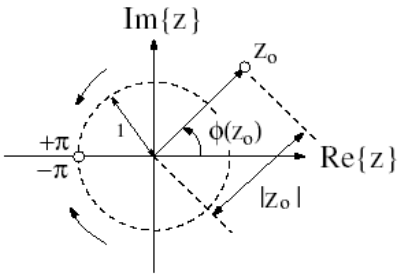
\includegraphics[width=0.4\textwidth]{Lezioni/Immagini/zeta}
	\vspace{-40pt}
\end{wrapfigure}

Data una frequenza bilatera $x(n)$ con $-\infty < n < \infty$ si definisce trasformata zeta:
$$X(z) = Z[x(n)] = \sum_{-\infty}^{\infty} x(n)z^{-n}$$
Esiste una corrispondenza biunivoca tra $x(z)$ e $x(n)$ e i loro domini solo se viene definita la regione di convergenza uniforme ROC, cioè i valori della variabile complessa $z$ tale che $x(z)$ è finita.

Nella regione di convergenza, $X(z)$ è una funzione analitica, cioè continua e indefinitamente derivabile con derivate continue in $z$.

La $z$ è una pulsazione complessa con dominio $\mathcal{C}$, rappresentabile in termini di modulo e fase come $z = \rho e^{j2\pi f} = \rho e^{j\omega}$. Si può ridurre a trasformata di Fourier discreta togliendo il coefficiente complesso e applicando la formula a una nuova sequenza. 

Deve valere la condizione di sommabilità in modulo, quindi la convergenza varia con la distanza e il piano si può dividere in circonferenze concentriche con comportamento diverso. 

La regione ROC dipende solo dal modulo $\rho$ delle pulsazioni complesse $z$, e non dalla loro fase: questo comporta le circonferenze come luoghi dei punti $z$ a modulo costante.
$$ \sum_{-\infty}^{\infty}\abs{x(n)\rho^{-n}} < \infty \implies  \sum_{-\infty}^{\infty}\abs{x(n)}\rho^{-n} < \infty$$
In particolare, è importante trovare i valori di $\rho$ che indicano la convergenza, e si ha che i valori sulla circonferenza di raggio unitario $\rho = 1$ sono i valori della trasformata di Fourier di frequenza 0. Quando c'è un ritardo, la regione sarà individuata con $[z \neq 0]$.

\begin{figure}[h]
	\centering
	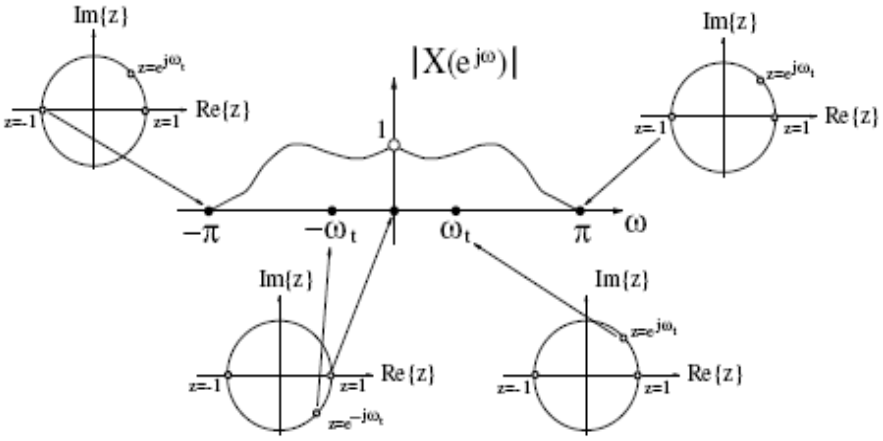
\includegraphics[scale=0.3]{Lezioni/Immagini/zdft}
\end{figure}

\subsection{Trasformate e ROC}
La trasformata zeta definisce una relazione biunivoca tra la sequenza $x(n)$ e una funzione della variabile complessa $z$. La biunivocità è garantita solo se si specifica la ROC di $X(z)$ e l'espressione analitica della trasformata.

Esistono relazioni specifiche tra la tipologia di una generica sequenza $x(n)$ e la ROC della relativa trasformata $z$:
\begin{itemize}
	\item Le sequenze $x(n)$ bilatere hanno supporto su istanti di tempo discreto negativi e positivi;
	\item Le sequenze causali possiedono coefficienti identicamente nulli per istanti di tempo negativi;
	\item Le sequenze anticausali possiedono coefficienti identicamente nulli per istanti di tempo positivi.
\end{itemize}

\subsubsection{Impulso $\delta$}
$$X(z) = \sum_{-\infty}^{\infty} \delta(n) z^{-n} = 1$$
Se l'impulso $x(n) = \delta(n)$ è una costante nel dominio trasformato, applicando la funzione zeta si ha un risultato simile: tutti i valori assumono 0 tranne quello per cui $n = 0$, quindi l'esponenziale diventa 1 così come tutta la trasformata. 

La regione di convergenza è costante e limitata a 1, e rappresenta tutto il piano complesso per cui la serie geometrica converge.
$$x(n) = 2\delta(n+1) + \delta(n) + 4\delta(n-2) = 2\sum_{-\infty}^{\infty}2\delta(n+1)z^{-n} + \sum_{-\infty}^{\infty}2\delta(n)z^{-n} + 4\sum_{-\infty}^{\infty}2\delta(n-2)z^{-n}$$
$$\implies 2z + 1 + 4z^{-2}$$
Il risultato è ottenuto scomponendo le sommatorie e trovando i valori per cui il numero all'interno delle parentesi si annulla. Bisogna sempre tenere conto del segno negativo dell'esponente.

\subsubsection{Gradino}
$$X(z) = \sum_{-\infty}^{\infty}u(n)z^{-n} = \sum_{0}^{\infty}z^{-n} = \sum_{0}^{\infty}\big(z^{-1}\big)^n = \frac{1}{1 - z^{-1}}$$
In una sequenza a gradino, la ROC corrisponde all'esterno della circonferenza di raggio unitario, cioè $\big[\abs{z^{-1}} < 1 \geq \abs{z} > 1\big]$. La stessa formula vale per il gradino anticausale, e la corrispondenza biunivoca si ritrova perché la ROC cambia in $\abs{z} < 1$.

\subsection{ROC per sequenze finite}
Le sequenze $x(n)$ con supporto finito sono i segnali a tempo discreto che possiedono un numero finito di coefficienti non nulli. Queste ammettono sempre una trasformata $X(z)$ esprimibile in forma chiusa come un polinomio composto da un numero finito di variabili del tipo $z^k$, $z^{-k}$ con $k$ intero.
$$X(z) = \sum_{n=-M}^{L} x(n)z^{-n}$$
\begin{wrapfigure}{R}{0.6\textwidth}
	% \vspace{-15pt}
	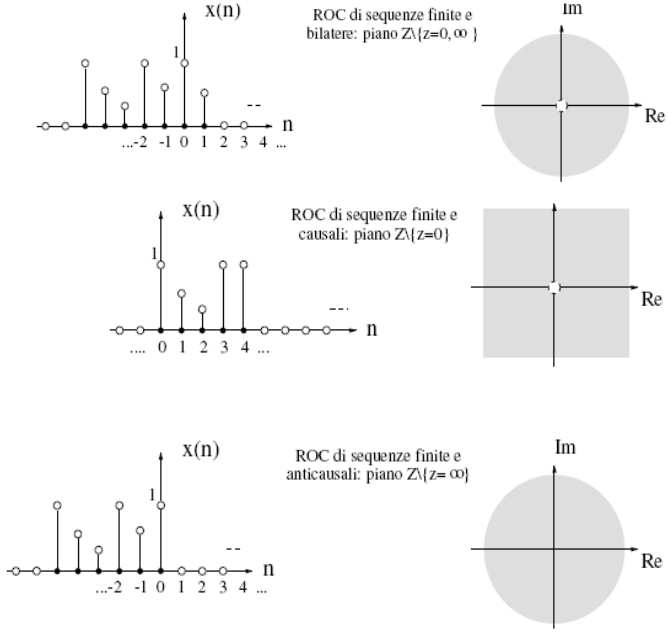
\includegraphics[width=0.6\textwidth]{Lezioni/Immagini/roc}
	\vspace{-40pt}
\end{wrapfigure}

La trasformata converge per qualunque $z$ nel piano complesso, eccetto il punto $z = 0$ se esistono termini del tipo $z^{-k}$ con $k > 0$, e il punto $z = \infty$ se esistono termini del tipo $z^{+k}$ con $k > 0$.

ROC per segnali bilateri di durata finita: intero piano complesso $\mathbb{C}$ tranne $[z = 0 \land z = \infty]$.

ROC per sequenze finite e causali: intero piano complesso $\mathbb{C}$ tranne $[z = 0]$.

ROC per sequenze finite e anticausali: intero piano complesso $\mathbb{C}$ tranne $[z = \infty]$.

Essendoci polinomi, sia il numeratore che il denominatore potrebbero annullarsi: nel primo caso si chiamano zeri, altrimenti poli. Per individuare i valori si può raccogliere i fattori arrivando all'ordine 1 nel denominatore.

In questo caso i campioni infiniti vengono rappresentati come rapporto finito di polinomi infiniti.

C'è una parte in comune $z = \alpha$ che annulla sia denominatore che numeratore, quindi gli zeri corrispondenti si semplificano e la sequenza resta finita. Ci sono $N - 1$ poli per $z = 0$.

Gli zeri si posizionano in modo uniforme a intervalli distanti uguali, nelle pulsazioni complesse. 

Serie geometrica:

In altre parole, sequenze causali = esterno della circonferenza, sequenze anticausali = interno.

L'importante è ragionare sui poli, che determinano la convergenza in base alla causalità. Il numero di poli e zeri corrisponde all'ordine, che può essere diverso tra numeratore e denominatore.

La frequenza è legata alla posizione angolare, quindi essendo i poli in zero la loro influenza si riflette su tutte le frequenze o nessuna: il contributo è nullo.

Studiando i poli si analizza la regione in cui la funzione viene amplificata e cresce in valore, gli zeri dove diminuisce. Insieme quindi danno l'andamento delle frequenze.

I coefficienti nell'equazione alle differenze corrispondono ai coefficienti nella trasformata, considerando il cambiamento di segno. Al numeratore c'è la parte non ricorsiva, e al denominatore quella ricorsiva. Se non c'è il denominatore, la sequenza è FIR.

Il sistema è stabile se la trasformata di Fourier è interna alla regione di convergenza. 

I sistemi FIR hanno risposta d'impulso limitata, e si può immediatamente passare alla rappresentazione tramite equazione alle differenze dato che i coefficienti sono gli stessi. I sistemi non sono ricorsivi.



\section{Equazioni alle differenze}
I LTI causali a tempo discreto possono essere rappresantati in modi differenti, tra cui la combinazione lineare con coefficienti costanti nel tempo (invariante). 

Il comportamento di un sistema LTI a tempo discreto e causale può essere descritto anche da equazioni alle differenze, come visto precedentemente:

Accumulatore: memoria infinita, generalmente si assegna un valore all'istante di partenza. 

Il ritardo sulla y indica di che ordine è il sistema: il primo ordine, per esempio, ha ricorsione con un campione in ritardo. 

La media cumulativa è un sistema ricorsivo non stazionario, con normalizzazione effettuata in base a un parametro non costante. 

La radice quadrata non è un sistema lineare: non esistono sommatorie, ma il termine y compare al denominatore quindi non è rappresentabile come combinazione lineare. 

La risposta all'impulso viene descritta attraverso la convoluzione, come sequenza finita o infinita. I primi non hanno la ricorsione, sono campioni combinati con pesi: i valori di h sono i coefficienti di x (bk). \\
Se la sommatoria va a infinito, non c'è una diretta corrispondenza con il dominio delle frequenze, quindi è inutile cercare y(n) guardando la risposta ma si utilizza il dominio trasformato.
\section{Sistemi LTI e trasformata zeta}
\subsection{Stabilità BIBO}
La stabilità BIBO di un sistema LTI impone che la risposta all'impulso $h(n)$ sia sommabile in modulo. Se il sistema è causale, la condizione si traduce nel dominio $z$ imponendo che la funzione di trasferimento $H(z)$ abbia poli contenuti nella circonferenza di raggio unitario del piano $z$. 

Le caratteristiche della sequenza dipendono dalla posizione dei poli: la convergenza, e conseguentemente la stabilità, sono determinate dall'appartenenza al cerchio unitario.

I poli all'esterno del cerchio $\abs{z} = 1$ ...
Poli multipli sul cerchio unitario conducono a una crescita di tipo polinomiale. 

Riassumendo:
\begin{itemize}
	\item Se il sistema è causale, condizione necessaria e sufficiente per la stabilità BIBO è che $H(z)$ abbia tutti i poli contenuti nella circonferenza di raggio unitario;
	\item ...
\end{itemize}

Quando il polinomio è espresso tramite potenze negative, se c'è una costante essa corrisponde all'assenza di ritardo, quindi sia al numeratore che al denominatore si somma 1 per indicare l'istante corrente. 

Tutte le volte che la soluzione non è a coefficienti reali, è presente il complesso coniugato. I monomi vengono espressi in termini di potenze negative di $z$.

\subsection{Filtri}
Avendo a disposizione la trasformata con i poli e gli zeri, conoscendo le proprietà di continuità della funzione analitica è possibile conoscere l'andamento delle frequenze.

Se un polo reale è molto vicino al cerchio di raggio unitario, si ha che il denominatore si annulla con valori prossimi a $\rho = 1$, ma a $z = 1$ c'è un picco e la risposta cresce in funzione alla posizione del polo. In altre parole, ogni polo ha un'influenza sulle frequenze a seconda della loro vicinanza.
 
Introducendo un fattore di normalizzazione $1 - \alpha$, è possibile confrontare i filtri con valore di picco (guadagno) unitario.

Per enfatizzare le basse frequenze, è sufficiente inserire degli zeri per farle crescere di valore. Creando monomi con radici e aggiungendole al numeratore e al denominatore, si creano filtri in grado di alzare o abbassare le frequenze manipolando le posizioni di poli e zeri.

Nella realtà bisogna considerare che è impossibile azzerare completamente una parte di frequenza, ma ci saranno delle oscillazioni più o meno ampie.

Tanto più i poli sono vicini all'asse reale, più influenzano le frequenze basse (filtro passa-basso).

Se la frequenza è causale, il numero di zeri non deve superare il numero di poli.
% foto sistemi
Ricostruendo la frequenza a partire dal filtro, si ha $H(z) = k \frac{z}{denz - \alpha} = \frac{k}{1 - \alpha z^{-1}}$ con $k$ costante. Se il guadagno è unitario, $\abs{H(z)_{f=0 \land z=1} = 1}$ da cui $k = 1 - \alpha$ (filtro con sempre la stessa altezza).

\subsection{Sistema inverso}
Un sistema inverso ha lo scopo di compensare i poli e gli zeri, ed è un sistema che inverte il comportamento di un altro sistema LTI tale che la risposta rimanga inalterata.

Il numeratore di uno dev'essere uguale al denominatore dell'altro e viceversa, e la funzione di trasferimento è pari a una costante unitaria nel piano $z$ (identità).




%\section{Immagini}
Un'immagine a colori viene percepita dal sistema visivo grazie all'impatto con le onde elettromagnetiche, caratterizzate dalla lunghezza d'onda $\lambda$ (proporzionale all'inverso della frequenza, $\lambda \propto \frac{1}{v}$) e dall'ampiezza (intensità). La lughezza d'onda è rapportata il periodo: indica quanto ci mette un ciclo a compiersi.

Lo spettro è in buona parte invisibile, con estremi alti che corrispondono alle radiazioni ultraviolette e bassi a radiazioni infrarosse. La porzione visibile è misurata in nanometri, con ordini di grandezza molto alti.

% arcobaleno

Il cristallino focalizza l'immagine sulla retina come una lente, e il colore è processato nella retina da coni e bastoncelli, in numerose tipologie con risposte differenti a seconda della lunghezza d'onda. Essi convertono le onde elettromagnetiche in uno stimolo elettrico.

I coni producono segnale per livelli di luminosità più alti, e possono essere:
\begin{itemize}
	\item L (long waves), sensibili al rosso;
	\item M (middle waves), sensibili al verde;
	\item S (short waves), sensibili al blu.
\end{itemize}

I bastoncelli funzionano con le rappresentazioni in toni di grigio, esono in percentuale estremamente maggiore; essendo essi atti a misurare la variazione d'intensità, gli esseri umani hanno più sensibilità in condizioni di scarsa luce. La percezione ultima del colore è legata a intensità e crominanza (tinta, saturazione), e le due dimensioni sono separabili. 

L'occhio è più sensibile alle variazioni di luce nel centro dello spettro visibile, quindi lo spettro avrà la forma di una curva con funzione che varia al variare delle lunghezze d'onda. A seconda dei nanometri della radiazione, alcuni coni saranno attivati, eventualmente fondendo le risposte: il colore è combinazione di contributi a diverse lunghezze (spettro).

% onde colore

\subsection{Segnale reale}
Per descrivere esattamente il segnale che forma l'immagine a partire da una scena occorre:
\begin{itemize}
	\item $E(\lambda)$, distribuzione spettrale dell'illuminante (SPD);
	\item $R(\lambda)$, riflettanza spettrale di ogni elemento della scena;
	\item $S(\lambda)$, sensitività dei recettori (coni e bastoncelli).
\end{itemize}

L'oggetto assorbe una parte della radiazione e ne ritrasmette un'altra parte (parametri legati alla capacità di riflettere), i cui segnali interferiscono con i recettori umani. La luce visibile è quindi $E(\lambda) \cdot R(\lambda)$, e ogni colore può essere descritto da tre parametri (RGB).

La maggior parte delle sorgenti luminose produce contributi di luce su più lunghezze d'onda:
$$L = \int E(\lambda) R(\lambda) l(\lambda) d\lambda$$
$$M = \int E(\lambda) R(\lambda) m(\lambda) d\lambda$$
$$S = \int E(\lambda) R(\lambda) s(\lambda) d\lambda$$
I numeri in output si definiscono valori di stimolo, che poi si traducono nei canali RGB. Le distribuzioni continue in funzione di $\lambda$ si trasformano in valori discreti in spazio tridimensionale grazie all'integrale.

Le immagine acquisite da una fotocamera digitale sono differenti da quelle elaborate dall'occhio umano: il sistema visivo viene simulato tramite sensori e processamento. Ogni camera ha una matrice che trasforma il segnale in modo da renderlo simile all'output del cervello, e i valori ottenuti dai sensori sono interpolati. 

I dati sono fatti passare in filtri colore, disposti secondo Bayer pattern. Il verde è il colore recepito meglio, e permette di misurare maggiormente le variazioni di intensità (e conseguentemente i dettagli dell'immagine). 

\subsection{Sintesi}
La somma dei contributi delle onde è chiamata sintesi additiva, e viene usata dai dispositivi che imitano l'occhio umano; esiste anche la sintesi sottrattiva, che fa differenze in base allo spettro e ai colori complementari di RGB (ciano, magenta, giallo). 

Quest'ultima consiste nella sovrapposizione di più filtri: il colore che giunge alla vista è quello che riesce a passare per tutti i filtri, dato che ognuno di essi sottrae una parte della luce che lo attraversa. 

% filtri

Esistono rappresentazioni che separano i canali in base alla loro intensità, mettendola in evidenza in base alla frequenza delle onde. Alcuni esempi di modelli sono:
\begin{itemize}
	\item RGB (red, green, blue), usato dalle camere e videocamere digitali;
	\item HSB (hue, saturation, brightness), corrisponde alla percezione umana del colore;
	\item HSV (hue, saturation, value), HSB con tinta definita su un angolo;
	\item CMYK (cyan, magenta, yellow, black), utilizzato per la sintesi sottrattiva nei sistemi di riproduzione;
	\item YIQ, per i segnali TV e VHS in America;
	\item YUV, per i segnali TV e VHS in Europa;
	\item YcbCr, per i video digitali.
\end{itemize}

Il formato grafico è la tecnologia utilizzata per memorizzare il file. Le immagini hanno due tipologie di formato: 
\begin{itemize}
	\item Raster, scalate in base a un numero prefissato di pixel e bit per pixel (bitmap) in una griglia di elementi, usate per digitalizzazione ed elaborazione di scene reali. L'accuratezza della rappresentazione dipende dal numero di pixel e dalla loro condifica (quantizzazione);
	\item Vettoriale, rappresentate con formule matematiche e oggetti, applicabili solo nel mondo geometrico ma con qualità maggiore. Le immagini sono più complesse e non viene persa definizione, ma sono più difficilmente modificabili.
\end{itemize}
Un'immagine in meta formato è una combinazione di questi formati, cioè contiene informazioni di ogni tipo: solitamente viene usato raster con alcuni elementi vettoriali.

\subsection{Risoluzione}
Le immagini hanno dimensioni espresse in pixel, mentre le dimensioni fisiche dipendono dal dispositivo di acquisizione. 

La risoluzione dà informazioni sulla quantità o la densità di pixel contenuti in un'immagine (ppi, pixel per inches). In caso di stampa o acquisizione con scanner si misura in dpi, dot per inches (gocce di inchiostro). Più alta è la risoluzione, più piccola è la dimensione fisica dei pixel: tipicamente una qualità alta di stampa ha una risoluzione intorno ai 300 ppi.

   
\subsection{Istogramma}
Un istogramma rappresenta l'insieme dei valori che un segnale può assumere, espresso in livelli di quantizzazione. Non dà informazioni spaziali, ma solo sul contrasto e sul numero di bit: indica quanti campioni assumono un certo valore (quantizzatore ottimo), e in base a ciò è possibile decidere come applicare la compressione (probabilità normalizzata).

HDR: usa n bit per catturare una porzione del range dinamico con differente esposizione, per poi sovrapporre tutte le immagini ottenute in modo da avere una visione più chiara. 

Per rappresentare meglio immagini con bianco o nero predominante, si utilizzano quantizzatori con pochi bit tagliando tutti i valori che non vengono utilizzati, in modo da avere una distribuzione più uniforme. 

Effettuando il dithering (evitare i salti), bisogna anche aggiungere rumore casuale: in questo modo le basse frequenze vengono nascoste dalle alte, e interferiscono con il rumore di quantizzazione.

\section{Audio}
Un segnale sonoro è la variazione di pressione sul timpano, percepito nel tempo attraverso l'aria (mezzo di propagazione). Il suono è un'onda di pressione come la luce, ma macroscopico.

L'aumento della frequenza non è linearmente in rapporto con l'ampiezza, ma si comporta seguendo una scala logaritmica. Il range di suoni in grado di essere percepite dagli umani è minore dell'insieme delle frequenze possibili, oltre esso ci sono ultrasuoni e infrasuoni. 

Le curve isofone rappresentano i suoni all'interno di una soglia di udibilità, che può essere superata fino al fastidio. 

Il segnale vocale può avere componenti fino a 10 KhZ, ma in genere se ne utilizzano solo 8, quindi questa è la frequenza di campionamento del segnale telefonico. 







\section{Audio}

 \begin{wrapfigure}{R}{0.4\textwidth}
	\vspace{-10pt}
	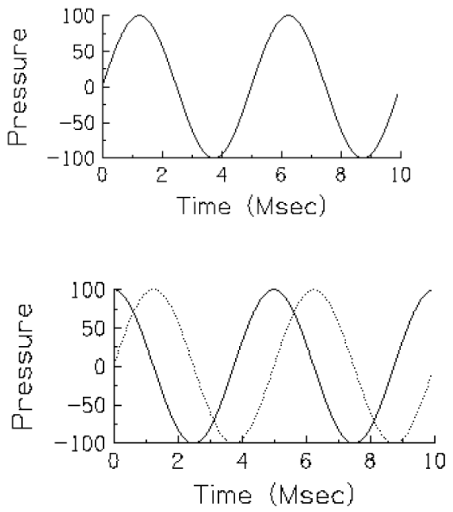
\includegraphics[width=0.4\textwidth]{Lezioni/Immagini/ondepressione}
	\vspace{-40pt}
\end{wrapfigure}

Un segnale sonoro è la variazione di pressione sul timpano, percepito nel tempo attraverso l'aria (mezzo di propagazione). 

Il suono è un'onda di pressione come la luce (fenomeno ondulatorio), ma macroscopico: le molecole dell'aria vengono compresse ed espanse, e la sorgente sonora vibra in modo longitudinale nella stessa direzione di propagazione del suono.
$$A(t) = A_{max} \cdot \sin(2\pi ft + \varphi_0)$$

I suoni elementari hanno andamento sinusoidale, periodico e con estensione indefinita. 

La maggior parte dei suoni natura sono caratterizzati da forme d'onda diverse, ma possono essere scomposte come una combinazione di suoni elementari.

Le componenti di un segnale sonoro sono individuate da:
\begin{itemize}
	\item Ampiezza $A$, che si misura rispetto al valore medio della pressione dell'aria ed è espressa in dB;
	\item Periodo $T$, la durata nel tempo di ogni ciclo dell'oscillazione, espresso in secondi;
	\item Frequenza $F$, velocità con cui i valori di pressione fluttuano ciclicamente, espressa in numero di cicli al secondo (onde e Hz).
\end{itemize}

Il valore 0 indicato sull'asse della pressione corrisponde al valore medio della pressione nell'aria. La differenza di fase ha unicamente a che vedere con il fatto che due funzioni siano diversamente allineate rispetto al tempo.

\subsection{Analisi di Fourier}
L'analisi di Fourier permette la rappresentazione del segnale sonoro nel dominio delle frequenze a partire dal tempo, esplicitando $f$.

\begin{figure}[h]
	\centering
	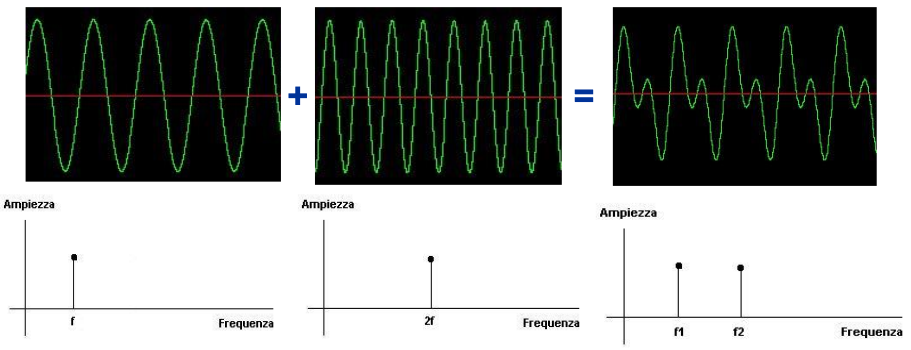
\includegraphics[scale=0.45]{Lezioni/Immagini/ondeverdi}
\end{figure}

La presenza di una linea nello spettro in frequenza indica la presenza di un segnale esattamente sinusoidale periodo, tuttavia i suoni caratterizzati da uno spettro discreto sono pochi. I suoni normalmente uditi hanno un inizio e una fine precisi, cioè sono contenuti in un intervallo temporale finito.

\begin{figure}[h]
	\centering
	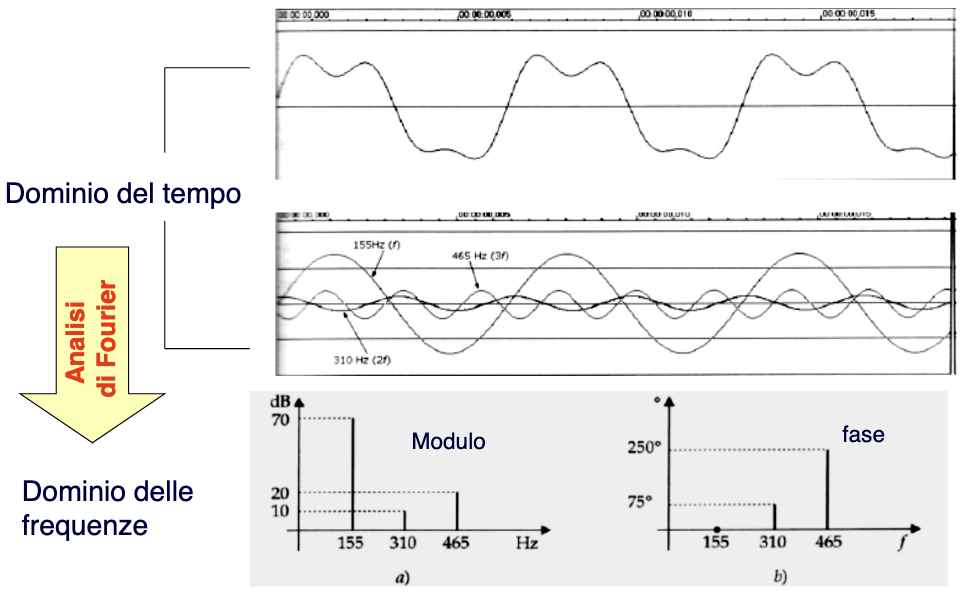
\includegraphics[scale=0.4]{Lezioni/Immagini/ondestorte}
\end{figure}

Ai parametri che descrivono un segnale ondulatorio possono essere associate le tre grandezze percettive che descrivono ogni suono:
\begin{itemize}
	\item Altezza, che rappresenta la tonalità dell'audio e ha come parametro la sequenza;
	\item Intensità, il volume, con parametro fisico l'ampiezza;
	\item Timbro, cioè la tipologia di strumento, con parametro fisico lo spettro.
\end{itemize}

A parità di frequenza fondamentale e intensità, due suoni possono differire per timbro (la sovrapposizione delle onde sinusoidali può essere diversa).

La frequenza fondamentale è proporzioanale all'altezza del suono, cioè della sensazione di acutezza o gravità. L'aumento della frequenza non è linearmente in rapporto con l'ampiezza, ma si comporta seguendo una scala di tipo logaritmico. Affinché in un suono sia possibile individuare un'altezza, esso deve essere periodico. 

\subsection{Grandezze fisiche e grandezze percettive}

 \begin{wrapfigure}{L}{0.4\textwidth}
	\vspace{-15pt}
	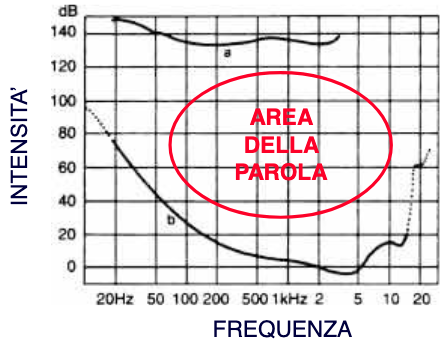
\includegraphics[width=0.4\textwidth]{Lezioni/Immagini/parola}
	\vspace{-40pt}
\end{wrapfigure}

Ampiezza e frequenza della forma d'onda hanno effetto sul suono percepito: variazioni di piccola ampiezza producono suoni di bassa intensità e viceversa, e al crescere della frequenza aumenta il tono (non linearmente).

Le energie in gioco nei fenomeni acustici sono irrilevanti rispetto a quelle nel fenomeno luminoso. 

Il range di suoni in grado di essere percepite dagli umani (tra i 20 e i 20.000 Hz) è minore dell'insieme delle frequenze possibili, oltre esso ci sono ultrasuoni e infrasuoni. 

Il volume aumenta man mano che l'ampiezza cresce, e l'incremento di tono è sempre più piccolo al crescere della frequenza.

Il campo di udibiltà è determinato dai valori limite di intensità e frequenza. Il limite inferiore per l'intensità è costituito dalla curva di soglia di udibilità, mentre quello superiore dalla soglia del dolore. 

Le curve isofone rappresentano i suoni all'interno di una soglia di udibilità, che può essere superata fino al fastidio. Esse dipendono dall'intensità e dalla frequenza.

Vengono usate scale di rappresentazione che riflettono uguali differenze percettive. La scala di Mei indica la relazione tra sensazione di altezza e frequenza, uguali differenze sulla scala corrispondono a uguali differenze percepite di tono ma non di frequenza.

Le ampiezze sono rappresentate in scala logaritmica e hanno come unità di misura il dB. Incrementi di 1 dB corrispondono a JND (Just Noticeable Differences).

\subsection{Campionamento}
Le variazioni di pressione vengono tradotte in variazioni di tensione/corrente elettrica dal microfono, che effettua una trasduzione elettroacustica. Il filtro antialiasing è applicato tramite amplificazione e filtraggio, per poi effettuare conversione A/D e registrazione su supporto.

La funzione a gradini generata dal convertitore viene filtrata con un filtro passa-basso prima del campionamento, per limitare le frequenze e l'aliasing. L'intervallo di frequenze che viene mantenuto dipende dall'applicazione.

Il segnale vocale può avere componenti fino a 10 KhZ, ma in genere se ne utilizzano solo 8, quindi questa è la frequenza di campionamento del segnale telefonico. Il segnale musicale ha range tra 20 Hz e 20 kHz.

Dopo la conversione DA, nell'output possono essere di nuovo presenti alte frequenze a causa del campionamento e della quantizzazione, quindi viene applicato un ulteriore filtro. La frequenza di campionamento standard è di 44,1 kHz, per registrare audio in formati differenti. Al di fuori di tale soglia si incorre in sovracampionamento o sottocampionamento (aliasing). 

La maggior parte dell'informazione del segnale vocale è contenuta in 4 kHz, ma esso andrebbe campionato a 40 kHz. Esiste anche per il campionamento il SNR (dB), con potenza del segnale proporzionale al quadrato della tensione.
$$SNR = 10\log_{10} \frac{V^2\text{segnale}}{V^2\text{rumore}} = 20\log_{10} \frac{V\text{segnale}}{V\text{rumore}}$$

\subsection{Dimensione e codifica}
Lo spazio in memoria (kB) occupato da un file audio si calcola con la seguente formula:
$$\frac{f_c \cdot D \cdot b \cdot N_c}{8 \cdot 1024}$$
$f_c$ è la frequenza di campionamento, $D$ è la durata in secondi, $b$ è il numero di bit del quantizzatore e $N_c$ è il numero di canali (mono o stereo).

I dati non compressi crescono al crescere della risoluzione del quantizzatore, dato che aumenta il numero di bit. Un segnale stereo raddoppia la banda per la trasmissione. 

La codifica può avvenire in due modi:
\begin{itemize}
	\item PCM (Pulse Code Modulation), modulazione del codice dell'impulso;
	\item PAM (Pulse Amplitude Modulation), modulazione dell'ampiezza dell'impulso.
\end{itemize}

La PCM converte in forma digitale i segnali analogici, trasformando le forma d'onda attraverso campionamento, quantizzazione e codifica. I valori numerici diventano e di 4 bit, e la rappresentazione può essere lineare o non.

Il trasmettitore digitale associa una forma d'onda a ogni cifra in uscita dal PCM, e all'uscita del canale le onde sono riconosciute dal ricevitore digitale e riconvertite nelle cifre originarie.

PAM è un modo per associare forme d'onda a simboli in uscita da una qualsiasi sorgente discreta. Essa prevede che si associ a ogni numero nella sequenza di bit la stessa pulsazione base, con un'ampiezza che dipende dal valore trasmesso.

I sistemi PAM inviano sul canale una sequenza di forme d'onda diverse tra loro, ma di diversa ampiezza. In ricezione, osservando l'ampiezza si può risalire al messaggio originale.

Nel processo di digitalizzazione, la qualità del suono è legata al tentativo di soddisfare due esigenze opposte:
\begin{enumerate}
	\item Fedeltà nella riproduzione;
	\item Dimensione del file.
\end{enumerate}

Le onde creano interferenze nello spazio, quindi è necessario creare l'effetto di più suoni generati in punti distinti e il numero di canali è un fattore importante. Le configurazioni più usate sono stereo e surround $5 + 1$, con 5 canali contenenti frequenze medie e alte, e un subwoofer per quelle basse. 

In fase di scrittura su disco, i campioni provenienti da diversi canali vengono trasmessi in successione. Questa tecnica si chiama interleaving, o multiplexing in caso di trasmissione. Al momento della riproduzione, occorre utilizzare buffer per la sincronizzazione.

\section{Video}
Un video viene percepito dal nostro sistema visivo con la \textbf{persistenza della visione}, e per ottenere il movimento apparente (serie di immagini statiche) è necessario individuare la frequenza minima per avere una visione continua. 

La persistenza della visione è un fenomeno per il quale un'immagine rimane per qualche frazione di secondo in memoria, attribuito a livello cerebrale. Ciò permette di ottenere un movimento continuo. 

Esistono frequenze di campionamento prestabilite per percepire una serie di immagini come un video continuo:
\begin{itemize}
	\item Una teleconferenza è a 10 fps;
	\item Un film muto è a 16 fps (\textit{limite del movimento a scatti});
	\item Un film sonoro è a 24 fps;
	\item Le televisioni sono a 25-60 fps, a seconda della tipologia.
\end{itemize}

Dalla conoscenza della risposta si determina la progettazione di un dispositivo di riproduzione video. La risposta dell'HVS dipende dal contenuto frequenziale, rispetto al tempo e allo spazio.

Per definire il numero di immagini al secondo (\textit{frame rate} e \textit{refresh rate}) bisogna definire una \textbf{soglia critica} legata alla frequenza di Flicker, ottenuta in base a una serie di parametri, quindi variabile nel tempo e nello spazio.

Se la frequenza è troppo alta, l'immagine non è più nitida: il range ha anche un limite superiore, con estremi tra i 20 e gli 80 Hz, definendo una \textit{Critical Flicker Frequency} alla quale lo stimolo passa da intermittente a continuo. Essa varia in funzione di:
\begin{itemize}
	\item Luminosità media del display;
	\item Luminosità dell'ambiente;
	\item Distanza dallo schermo.
\end{itemize}

Un \textbf{video field} è un insieme di campioni in un'immagine, composto da linee alternate. I vari field sono campionati a istanti diversi. L'aumento delle frequenza di refresh per la televisione è ottenuto dividendo l'immagine in due campi, le cui righe non vengono scansionate sequenzialmente ma sono \textbf{alternate tra pari e dispari}. Il refresh include anche la ripetizione della stessa immagine, riducendo il flicker.

La \textbf{scansione progressiva} consiste nella trasmissione in sequenza e in modo continuo di tutte le linee. Al contrario, la \textbf{scansione interlacciata} divide il frame in field trasmessi in metà del tempo totale.

I 24 fps del cinema non sono sempre sufficienti, quindi i proiettori possono arrivare a 48 o addirittura 72. Nella trasmissione analogica, invece, la frequenza viene virtualmente raddoppiata con l'interfacciamento: le risposte in frequenza vengono combinate. Nei display dei computer si utilizza un rate di 72 fps.

Il sottocampionamento introduce aliasing quando il movimento è molto veloce, causando differenze di percezione ovviate da opportuni filtri passa-basso (\textit{smoothing}). 

\subsection{Riproduzione}
Un segnale \textit{analogico} ha risoluzione definita dal \textbf{numero di linee di scansione}. \\
Un segnale \textit{digitale} ha risoluzione definita dal \textbf{numero di pixel}.

La riproduzione del colore cambia a seconda dello spazio, delle modalità di trasmissione e della quantizzazione per il segnale digitale. Bisogna rappresentare il colore mantenendo un segnale di luminanza compatibile, le stesse temporizzazioni e la stessa banda.

Per codificare le immagini, si cambia spazio colore in modo da separare luminanza da crominanza. Non ci sono limitazioni relative ai canali e ai componenti sulla stessa portante. 

 \begin{wrapfigure}{L}{0.35\textwidth}
	\vspace{-5pt}
	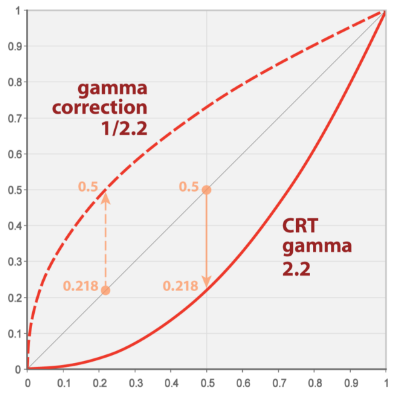
\includegraphics[width=0.35\textwidth]{Lezioni/Immagini/gamma}
	\vspace{-30pt}
\end{wrapfigure}

Il video fornisce informazioni sulla luminosità dell'immagine usando un segnale di luminanza $Y$ ottenuto sommando in modo pesato le componenti RGB, a cui viene in seguito applicata una correzione gamma. 
$$ Y = 0.299R + 0.587G + 0.114B$$
La maggioranza del segnale è composta dal verde; l'informazione colore è codificata in due canali aggiuntivi, ottenuti sottraendo la luminanza dalle componenti rosso e blu.
$$ U = 0.492(B - Y) \qquad V = 0.877(R - Y)$$

Queste due componenti sono chiamate \textbf{chrome}, e la rappresentazione di un valore indipendente dalla luminanza è definita crominanza. 

I coefficienti associati a ogni colore cambiano in base alla posizione geografica per lo standard analogico, mentre per il digitale è globalmente YCrCb. Nella combinazione lineare, il canale più importante è quello del verde. 

I più importanti standard di video analogico sono NTSC in Nord America e Giappone, PAL e SECAM in Europa. I segnali analogici usati sono YUV e YIQ. Le informazioni su colore UV e IQ sono combinate insieme in un segnale di chroma, che a sua volta è combinato con la luminanza Y.

Un altro aspetto da considerare è la \textit{dipendenza tra l'intensità del monitor e la tensione}, la quale ha un fattore esponenziale: il monitor tende a comprimere gli scuri, mostrandoli in livello maggiore.
$$B_d = v_d^{\gamma_d} \qquad \begin{cases}
v_d = \text{tensione} \\
B_d = \text{brightness} \\
\gamma_d = \text{gamma}
\end{cases}$$

Per questo motivo si utilizza la \textbf{gamma correction}, che aumenta l'intensità dei grigi. Essa compensa le caratteristiche di \textbf{non linearità} dei display, per mantenere la compatibilità con i televisori in bianco e nero.

Se il valore del canale rosso è $R$, lo schermo emette una luce proporzionale a $R^\gamma$, con $\gamma \approx 2.2$. In genere il segnale normalizzato viene corretto prima della trasmissione, elevando a $\nicefrac{1}{\gamma}$.

L'HDTV (alta definizione) è concepita per avere una risoluzione doppia rispetto alla TV analogica, con dimensioni in pixel molto più grandi che però permettono l'adattamento agli standard precedenti, aumentando il refresh rate. 

Poiché il sistema visivo è più sensibile all'intensità luminosa che alla croma, si riduce la risoluzione spaziale delle componenti cromatiche. Il campionamento del colore è espresso come $x : y : z$, dove:
\begin{itemize}
	\item $x$ è il numero di campioni di luminanza;
	\item $y$ è il numero dei campioni di chroma per ogni linea dispari;
	\item $z$ è il numero di campioni di chroma per le altre linee.
\end{itemize}

Nella digitalizzazione, i canali Cr e Cb sono di solito campionati orizzontalmente. Lo schema di sottocampionamento $4 : 4 : 4$ indica che non c'è sottocampionamento sulle componenti cromatiche, quindi i valori YCbCr sono tutti trasmessi. 

Per eliminare le coppie, si utilizzano schemi del tipo $4 : 2 : 2$ oppure $4 : 1 : 1$, che trasmettono solamente alcuni valori campionando orizzontalmente. 

 \begin{wrapfigure}{R}{0.4\textwidth}
	\vspace{-20pt}
	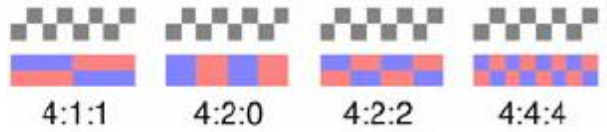
\includegraphics[width=0.4\textwidth]{Lezioni/Immagini/pixel}
	\vspace{-20pt}
\end{wrapfigure}

La compressione JPEG usa $4 : 2 : 0$, il quale elimina un fattore 2 in entrambe le dimensioni posizionando fra righe e colonne un pixel con croma media. Per ogni 4 campioni di luminanza, ci sono 2 chroma sulle linee dispari. 

\section{DCT wavelets}
L'obiettivo dell'analisi è la riduzione delle ridondanze, spostandosi in uno spazio dove le informazioni e i canali sono separati. 

Nel dominio diretto le componenti di un segnale $X$ sono tra loro significativamente correlate, quindi la stessa informazione è ridondante. Spostandosi nel dominio trasformato $Y = T[X]$, si cerca una rappresentazione dove le componenti siano molto meno correlate.

$Y$ può essere codificato in modo più efficiente di $X$, utilizzando solo le componenti del segnale che descrivono l'informazione. Lo spettro, per esempio, ha un contributo maggiore espresso con le basse frequenze al centro, quindi è possibile codificare solo una porzione determinata di energia.

In termini di compressione, sono necessari solo i bit delle componenti da tenere. Il modello di compressione permette di quantizzare con perdite trascurabili, in un cambio di spazio secondo due strategie:
\begin{itemize}
	\item Codificatore di sorgente, che riduce le ridondanze;
	\item Codificatore di canale, che incrementa l'immunità al rumore.
\end{itemize}

\subsection{Codifica con trasformate}
Questo algoritmo introduce perdita ed è computazionalmente costoso, a causa del calcolo delle trasformate. Una trasformata lineare e reversibile è usata per il mapping dell'immagine in un set di coefficienti che vengono poi quantificati e codificati.

Il mapping può essere effettuato secondo diverse metodologie, a seconda della capacità di decorrelazione dei dati, semplicità di realizzazione e altri fattori.

La KLT (analisi alle componenti principali) è la trasformata ottima, ma è computazionalmente inefficiente. DCT, invece, approssima il comportamento ottimo, ed è usata negli algoritmi di codifica più utilizzati (jpeg, mpeg).

La trasformata wavelet permette la multirisoluzione (jpeg2000), e funziona secondo il principio di determinazione di Heisenberg, trovando un compromesso tra le frequenze e il dominio temporale lavorando con tradeoff.

Data una funzione $f(x)$, la sua DFT $F(u)$ è:
$$F(u) = \frac{1}{M} \sum_{x=0}^{M- 1}f(x)e^{-j\frac{2\pi}{M}ux} = \frac{1}{M} \sum_{x=0}^{M- 1}f(x)g(u, x)$$
$$g(u, x) = e^{-j\frac{2\pi}{M}ux}$$

La trasformata è lineare e invertibile, e $g(u, x)$ è detto kernel della trasformazione diretta, da cui dipendono le proprietà. I kernel devono essere invertibili, lineari e separabili.

Trasformata di Fourier discreta 1D:
$$e^{-j\frac{2\pi}{M}ux} = \cos\big(\frac{2\pi}{M}ux\big) + j\sin\big(\frac{2\pi}{M}ux\big)$$
% immagine onde quadrate
Il segnale di partenza è proiettato in base al suo tempo e spazio con le sue parti reale e immaginaria. Seno e coseno hanno simmetria rispettivamente dispari e pari, e trasformando si osserva l'influenza di ciascuna componente. 

La trasformata coseno discreta (DCT) è lineare, con kernel diretto uguale a quello inverso (simmetria speculare), separabile e simmetrico. La componente continua è legata al valore medio dell'immagine (0, 0). 
$$T(u) = \sum_{x=0}^{M- 1}f(x)g(u, x) \qquad g(x, u) = \alpha(u) \cos\Big[\frac{(2x + 1)\pi u}{2N}\Big]$$
% immagine coseno
$$\alpha(u) = \begin{cases}
\sqrt{\frac{1}{N}} & u = 0 \\
\sqrt{\frac{2}{N}} & u = 1, 2, \dots, N - 1^{}
\end{cases}$$

La separabilità permette di calcolare la trasformata 2D tramite applicazioni successive della trasformata 1D alle righe e alle colonne, senza perdita di informazione. Ciascun blocco è costituito da $N \times N$ sottoblocchi.

Una maggiore quantità di informazione è presente nei primi coefficienti della DCT, rispetto allo stesso numero di coefficienti della DFT.
% dct vs dtf
Visualizzando un'immagine su un monitor con un range elevato (scala logaritmica), non si vede nulla perché il monitor arriva solo fino a 256.

\subsection{Analisi multirisoluzione}
Le immagini sono generalmente costituite da regioni connesse che formano gli oggetti, omogenee rispetto a una qualche proprietà.

L'analisi multirisoluzione permette di mettere in evidenza sia le immagini a bassa frequenza che quelle ad alta, con segnali e campioni di dimensioni diverse, concentrandosi su differenti posizioni nello spettro. 

Le caratteristiche locali di un'immagine sono contraddistinte da variazioni statistiche locali, dovute  discontinuità fra regioni omogenee. Caratteristiche nascoste a una data risoluzione possono essere individuabili a un'altra.

La tecnica più frequente è l'analisi piramidale, che parte dalla risoluzione massima e progressivamente sottocampiona, evidenziando i cambiamenti tra i dettagli e le perdite tra un livello e l'altro ricostruendo ogni volta l'immagine con meno dettagli. I pixel mancanti vengono approssimati tramite wavelet.

Il segnale è decomposto in un insieme di sottosegnali (sottobanda, analisi), passando attraverso filtri complementari, ciascuno dei quali agisce su una fascia di frequenze. Ricampionando, filtrando e ricombinando le sottobande (sintesi) si ottiene un'approssimazione $\hat{x}(n)$ dell'originale, non incorrendo in aliasing. 

Ciascuna sottobanda $(y_0(n), y_1(n))$ è ottenuta filtrando con un passa-banda $(h_0(n), h_1(n))$ il segnale originale. Poiché la sottobanda ha spettro limitato e pari a metà dell'originale, è possibile sottocampionare senza perdita di informazione. 
% immagine
%% da qui
Imponendo $\hat{x}(n) = x(n)$, si trovano le opportune coppie di filtri di sintesi e corrispondenti filtri di analisi che garantiscono una perfetta ricostruzione. In caso di più dimensioni (separabili), possono esserci $n$ filtri per righe e colonne che mettono in evidenza diverse porzioni di frequenze rispetto alla direzione. Flitraggio e sottocampionamento avvengono quindi in due fasi successive.

Si ottengono 4 immagini di output: $dV(m, n)$, $dH(m, n)$, $dD(m, n)$ le immagini nelle 3 dimensioni per le alte frequenze, e $a(m, n)$ l'immagine approssimata. Ciascuna sottobanda a sua volta può essere scomposta in 4 ulteriori sottobande.
% sottobande
Visivamente, è immediata la correlazione fra filtri di analisi e sintesi corrispondenti: sono ortonormali, cioè ortogonali a norma unitaria, e permettono una ricostruzione error-free in ciascun livello che a sua volta viene approssimato.

Dato che le statistiche locali sono facilmente modellabili e presentano molti valori nulli, questa codifica è particolarmente vantaggiosa per la compressione: non tutto l'istogramma viene occupato, oppure ci sono poche alte frequenze che possono essere eliminato. L'approccio di denoising per ridurre il rumore è utilizzato nelle applicazioni mediche.

Nell'analisi multirisoluzione, il filtro passa-basso è una funzione di scala (MRA), mentre il passa-alto è una wavelet generata a partire da una wavelet madre. Ogni approssimazione differisce dalla più vicina di un fattore 2.

Le wavelet descrivono la differenza di informazione fra due approssimazioni adiacenti. La formula in notazione monodimensionale è:
$$f(x)  = \frac{1}{\sqrt{M}} \sum_{k} W_\varphi (j_0, k) \varphi_{j_0, k} (x) + \frac{1}{\sqrt{M}} \sum_{j=j_0}^{J}\sum_{k} W_\psi(j, k)\psi_{j, k}(x)$$
$\varphi(x)$ è la funzione di scaling, con i relativi coefficienti di approssimazione. $\psi(x)$ è la wavelet madre, con i relativi coefficienti di dettaglio.

Tramite imposizione di equivalenze tra prodotti, è possibile misurare le variazioni lungo le righe, le colonne e le diagonali. Trasformando con la wavelet, è possibile pesare ogni contributo per capire quali frequenze e bande hanno influenza maggiore, valutando le features che caratterizzano l'immagine. 
% wt in 2 dimensioni
Per calcolare gli edge, si ha il segnale di partenza in una somma di contributi: la parte interessata (per esempio il filtro passa alto $\psi$) viene tenuta applicando la formula, mentre le altre componenti vengono annullate. 

Annullando anche i termini di edge orizzontali a tutte le scale e ricostruendo (sintesi) a partire da questi dati, si isolano i soli edge verticali.

Un altro approccio è il denoising, a partire dalle wavelet. La ricostruzione è effettuata dopo aver posto una soglia alta sui coefficienti a tutte le risoluzioni, accettando solo i valori al di sopra. 

L'immagine originale è una risonanza magnetica con un rumore bianco additivo o moltiplicativo, a cui viene applicata la procedura di denoising:
\begin{enumerate}
	\item Scelta della funzione wavelet;
	\item Scelta del numero di livelli;
	\item Sogliatura dei coefficienti di wavelet ed eliminazione di quelli inferiori alla soglia;
	\item Ricostruzione a partire dall'immagine approssimata all'ultima scala.
\end{enumerate}

Riducendo il rumore, si ha notevole perdita di dettaglio anche sugli edge, applicando soglie a tutte le risoluzioni. Agendo solo sulla risoluzione massima, si ha una perdita minore.

Per il principio di indeterminazione di Heisenberg, la distanza per ogni punto esatto di una funzione è infinitesima: pertanto, la risoluzione nelle frequenze è indefinita. Nel dominio trasformato, è nota l'informazione per ogni valore di $f$, ma $\delta x$ è infinito. 

In altre parole, in base al dominio, una dimensione è indeterminata. Il prodotto delle due, che corrisponde all'area, è sempre maggiore di un valore $K$:
$$\delta t \times \delta v \geq K$$
Nelle wavelet, è possibile determinare precedentemente una delle due dimensioni, avendo contemporaneamente informazione spaziale e frequenziale.

\section{Tecniche di compressione}
Il costo di un segnale dipende da campionamento e quantizzazione, fino ad arrivare a una quantità troppo elevata di dati per la memorizzazione ad alta qualità.

Per rappresentare l'informazione si ricorre alla compressione, cioè la trasformazione in un insieme di dati statisticamente incorrelati che garantiscano un grado di fedeltà (qualità) rispetto all'originale, e abbiano un accettabile peso computazionale per il tipo di applicazione.

Le tecniche di compressione si dividono in due grandi famiglie: lossy (con perdita accettabile a seconda dell'applicazione) e lossless (senza perdita). I dati ridondanti vengono rimossi, e il risparmio viene misurato tramite un rapporto di compressione in bit, dipendente appunto dalla ridondanza. 

I dati sono gli strumenti tramite i quali è rappresentata l'informazione, e quest'ultima può essere associata a diversi quantitativi di dati. Il principio della compressione è appunto minimizzare il numero di bit utilizzati. 
$$\text{rapporto di compressione } C = \frac{b_1 \text{ bit prima della compressione}}{b_2 \text{ bit dopo la compressione}}$$
$$\text{ridondanza relativa } R = 1 - \frac{1}{C}$$
Se $b_1 = b_2$, allora $R = 0$ e non ci sono dati ridondanti tra le due rappresentazioni. Un rapporto tipico di compressione è $10 : 1$, con corrispondente ridondanza $0.9$.

\subsection{Ridondanza}
Possono essere individuati diversi tipi di ridondanza, di cui almeno uno va ridotto:
\begin{enumerate}
	\item Della codifica;
	\item Spaziale o temporale (correlazione inter-campione);
	\item Percettiva, imponendo quantizzazioni più o meno spinte.
\end{enumerate}

I primi due consistono nella ridondanza statistica: i vicini possono essere correlati o dipendenti, quindi una parte dell'informazione è ripetuta. 

\subsubsection{Ridondanza della codifica}
La ridondanza della codifica non introduce perdita, quindi è reversibile e ha una soglia massima di compressione che può essere raggiunta. Quest'ultima dipende dal tipo di segnale.

L'idea è costruire un quantizzatore che venga usato nel miglior modo possibile, distribuendo i valori in modo equiprobabile tra i livelli. Alcuni livelli, secondo l'istogramma a livelli di grigio, hanno una maggiore probabilità di essere occupati, quindi è possibile calcolare quanto comprimere in base al numero medio normalizzato di bit necessari per ogni frequenza.

Se i valori sono sbilanciati, si ricorre alla codifica a lunghezza variabile, con numero di bit medio necessario per descrivere l'immagine:
$$L_{avg} = \sum_{k=0}^{L-1}l(r_k)p_r(r_k)$$
$l(r_k)$ è il numero di bit necessario per descrivere il $k$-esimo livello $r$, con frequenza (probabilità) $p_r$. Essendo gli standard a 256 livelli di grigio, la frequenza sarà costante e la sommatoria sarà 1, pertanto le immagini saranno codificate a $M\times N \cdot 8$ bit.

VLC (Variable-Length Coding) è una strategia di riduzione della ridondanza che impiega un numero minor di bit per rappresentare i livelli più probabili, e viceversa. Il numero medio di bit è minore rispetto alla lunghezza fissa.

\subsubsection{Ridondanza spaziale}
Quando l'istogramma è uniforme, però, la VLC non ha effetto. Tutti i valori sono equiprobabili, ma ciò li rende fortemente correlati (e pertanto ridondanti) spazialmente. Questo succede per esempio in immagini a righe, mentre lungo le colonne i valori sono incorrelati.

Si può ridurre la ridondanza spaziale individuata introducendo coppie run-length: il primo componente della coppia individua l'intensità, mentre il secondo il numero di volte con cui si ripete. L'approccio è lossless.

\subsubsection{Ridondanza percettiva}
L'immagine è percepita come se avesse un valore di grigio uniforme, ma l'istogramma è discordante da questa rappresentazione.
% immagine
Le informazioni ignorate dal sistema visivo umano possono essere eliminate, sostituite da un valore medio. Il processo è eseguito tramite quantizzazione, ma c'è perdita. 

\subsection{Entropia}
L'entropia è la misura della quantità di dati minima necessaria per codificare senza perdita una sorgente di informazione, modellando la sorgente come processo probabilistico con eventi statisticamente indipendenti.

Informalmente, rappresenta il valore dell'informazione attraverso incertezza e probabilità di un certo simbolo. La sorgente deve emettere valori tra di loro incorrelati, quindi non deve avere memoria. 

Nel caso delle immagini, c'è molto spesso dipendenza tra pixel contigui, ma l'entropia è la soluzione ottima a cui avvicinarsi il più possibile.

Un evento casuale $E$ con probabilità $p(E)$ ha un grado di incertezza (e una quantità di informazione) pari a:
$$I(E) = \log \frac{1}{p(E)}$$
La base del logaritmo dipende dall'unità di misura dell'informazione, in questo caso 2 (bit). Se un evento è certo, l'incertezza è nulla. 

Essendo l'entropia proporzionale all'incertezza, l'entropia di una sorgente con alfabeto $S = \{s_1, s_2, \dots,s_M\}$ è:
$$H(S) = \sum_{k=1}^{M} p_k \log_2 \frac{1}{p_k} = -\sum_{k=1}^{M}\log_2p_k$$
$p_k$ è la probabilità del $k$-esimo simbolo dell'alfabeto, e $\log_2\frac{1}{p_k}$ è la quantità di informazione contenuta nel simbolo $s_k$, cioè il numero di bit necessario per la codificaLa . situazione di equiprobabilità genera entropia massima.

L'entropia indica pertanto un limite inferiore (valore medio) per il numero di bit necessari per codificare un certo alfabeto, ipotizzando l'equiprobabilità di ogni livello e fornendo un punto di riferimento per i codici a lunghezza variabile. 

L'obiettivo di VLC è trovare il codice di lunghezza minima per descrivere il segnale. Se un codice $c_1, c_2, \dots, c_M$ ha parole con lunghezza $b_1, b_2, \dots, b_M$, il numero medio di bit richiesti è:
$$R = \sum_{k=1}^{M}b_kp_k$$
Il problema della progettazione di codice è la ricerca di parole con lunghezza media vicina all'entropia della sorgente del segnale, cioè $r$ vicino a $H$, e la stima della precisione dei valori di probabilità.

La massima entropia implica un contenuto informativo visivo basso, essendo i valori equiprobabili. Immagini diverse possono avere entropia simile, ma essa serve come valore di riferimento solo con sorgenti senza memoria, quindi il rapporto di compressione può essere molto differente in caso di fotografie o immagini con pattern.

\subsubsection{Codici di Huffman}
todo

Se il segnale viene letto sequenzialmente, non si hanno informazioni precise riguardo alla distribuzione dei simboli: essa viene stimata tramite strumenti che aggiornano a ogni valore la possibile frequenza.

\subsection{RLC}
La correlazione tra bit può portare a un elevato risparmio, ma per ottenerla si deve ricorrere a sorgenti con memoria. 

Il segnale si presenta con tanti 0 in sequenza intervallati da 1, e viene trasmessa la coppia di valore assunto e numero di valori (run-length coding). 

Questa tecnica è impiegata per la codifica di immagini a colori, ma è poco efficiente per immagini reali a causa delle imprecisioni e del rumore. 

Il bitmap prevede una modalità di compressione senza perdita utilizzando appunto RLC, codificando le informazioni sequenziali ripetute. Il rapporto di compressione può essere minore di 1 in caso che nuovi bit vengano sprecati per creare coppie di valori diversi da quelli non contigui.

\subsection{Differential coding}
Questa tecnica viene applicata quando RLC è inefficiente, e ha come scopo la riduzione della ridondanza in simboli consecutivi di un datastream.

Osservando il segnale in termine di differenza tra frequenze, una forte correlazione spaziale viene sfruttata tramite codifica a lunghezza variabile sui picchi dell'istogramma. 

Viene calcolata la differenza tra frequenze adiacenti, ed essa viene codificata. Il segnale viene ricostruito sommando le differenze a partire dal valore iniziale (noto).

Per sfruttare la ridondanza tenendo conto delle differenze, è possibile anche sfruttare la differenza tra il valore attuale e quello predetto. Se la regione è uniforme in base a determinate regole, sarà immediato il calcolo del valore successivo, sfruttando l'interpolazione. 

La differenza, con valori accurati, tenderà a 0 con un istogramma stretto, e di conseguenza un'entropia minore (MPEG). 

\subsection{Algoritmi lossless}
Lossless JPEG non usa la DCT e non introduce perdita tramite codifica predittiva, sfruttando l'uniformità delle regioni.

Gli algoritmi lossless universali non richiedono la conoscenza a priori della distribuzione di probabilità dei simboli: in genere riescono a modellare dinamicamente le caratteristiche dei dati, adeguando la codifica.

Viene aggiunto un ulteriore bit nel dizionario che permette di identificare l'occorrenza dei valori. Tutte le volte che un valore si ripete, la codifica può essere riutilizzata usando la coppia e associandola a un livello (analisi delle frequenze). 

In funzione di com'è costruita l'immagine, ciascun algoritmo sarà più o meno efficiente. 

\subsection{Codifica video}
Nei video esiste una correlazione non solo tra i pixel dello stesso fotogramma, ma anche tra fotogrammi adiacenti. In base alla ridondanza, è possibile applicare compressione spaziale e temporale.

La codifica predittiva rimuove entrambe le tipologie, con un errore di predizione $e(n)$ ottenuto tramite VLC e diversi modelli di predizione. % immagine

In presenza di un segnale sonoro a una generica frequenza, si ha un'alterazione della soglia di udibilità per le frequenze limitrofe al segnale, che non vengono percepite. 

% slide 47



\section{Approcci basati su parsimonia}
I due problemi confrontati consistono nella grande e piccola parsimonia, risolti con gli algoritmi di \textbf{Fitch} e \textbf{Sankoff}.

Il criterio di parsimonia si basa sul concetto di \textit{rasoio di Occam}, cioè la scelta della soluzione più semplice. L'albero dovrebbe avere la massima verosimiglianza, ma il modello di evoluzione sottostante dev'essere statistico e i tempi di calcolo sono elevati.

\subsection{Grande parsimonia}
Il \textbf{problema della grande parsimonia} consiste nel trovare la filogenesi (l'albero, sconosciuto) che minimizzi il numero di cambiamenti di stato, il momento in cui un carattere viene acquisito. In questo caso la matrice non è binaria, perché ogni carattere può avere più stati, non necessariamente in sequenza.

NB: il problema in versione semplificata considera solo caratteri presenti o meno, quindi la matrice corrispondente è binaria e ogni valore può essere solo 0 o 1.

Questo algoritmo è NP-completo, però può essere ridotto al \textbf{problema della piccola parsimonia}, in cui l'istanza in input è data dalla matrice $M$ e dalla topologia dell'albero. Si vuole determinare quale specie etichetta ogni foglia, e quali passaggi di stato sono rappresentati da ogni arco. 

\subsection{Piccola parsimonia}
La differenza tra la piccola e la grande parsimonia è che nella prima in input c'è la topologia dell'albero, quindi il problema è solo l'etichettatura.

Questo problema, in altre parole, consiste nel riempire l'albero a partire dalla struttura. Esso ha come istanze:
\begin{itemize}
	\item Una matrice triangolare $M$ con $n$ specie e un insieme di caratteri $C$;
	\item Un albero $T$, le cui foglie corrispondono alle specie di $M$;
	\item Per ogni carattere $c \in C$, un costo $w_c$ fra ogni coppia di stati.
\end{itemize}
Una soluzione ammissibile è un'etichettatura $\lambda$ che assegna a ogni nodo uno degli stati possibili per i caratteri $C$. \\
La nostra funzione obiettivo andrà quindi minimizzata:
\begin{equation*}
	min \sum_{c \in C} \sum_{(x, y) \in E(T)} w_c(\lambda_c(x), \lambda_c(y))
\end{equation*}
dove $E(T)$ è l'insieme dei lati di $T$.

\begin{example}{Piccola parsimonia}{}

Si ha in input una matrice $N$ di questo tipo: 
\smallskip
\begin{center}
\begin{tabular}{l | *{6}{c}}
	\# arti & 0 & 1 & 2 & 4 & 6 & 8 \\
	\hline
	0 & 0 & 1000 & 2000 & 4000 & 6000 & 8000 \\
	1 & ~ & 0 & 60 & 150 & 190 & 232 \\
	2 & ~ & ~ & 0 & 30 & 70 & 120 \\
	4 & ~ & ~ & ~ & 0 & 25 & 80\\
	6 & ~ & ~ & ~ & ~ & 0 & 10\\
	8 & ~ & ~ & ~ & ~ & ~ & 0
\end{tabular}
\end{center}
\smallskip
Si indica che il costo di passare da $0$ a $1$ arto è elevato, da $0$ a $2$ arti ancora più elevato, da $6$ a $8$ arti invece è meno elevato, eccetera (in pratica, si assegna un costo legato al numero di arti che la specie aveva prima e dopo essersi evoluta, completamente inventato). È un esempio di caratteri non binari, possono avere più stati. Una matrice di questo tipo è \textit{parte dell'istanza}. \\

\begin{center}
\begin{tabular}{l | c c}
	M & \# arti & Gene X \\
	\hline
	Topo & 4 & 0 \\
	Uomo & 4 & 0 \\
	Ragno & 8 & 1 \\
	Mosca & 6 & 0 \\
	Antilope & 4 & 0
\end{tabular}
\end{center}

\begin{center}
\begin{forest}
	for tree={
		circle, draw, 
		minimum size=1.5em,
		s sep=1cm
	},
	[~, fill=gray,
		[~, fill=red,
			[~, nodevalue={south}{Mosca}],
			[~, nodevalue={south}{Ragno}]
		],
		[~, fill=green,
			[~, nodevalue={south}{Uomo}],
			[~, nodevalue={south}{Topo}],
			[~,nodevalue={south}{Antilope}]
		]
	]
\end{forest}
\end{center}

Nella piccola parsimonia bisogna capire qual è l'etichettatura dei nodi interni (grigio, rosso e verde) in modo che la \textit{somma totale dei costi su ogni arco sia minimizzata}. Si possono trattare separatamente ogni singolo carattere, poiché questi sono \textbf{indipendenti}, quindi l'algoritmo è scritto in maniera tale da trattare un carattere per volta.

\end{example}

\subsection{Algoritmo di Sankoff}
Questo è un algoritmo risolutivo per il problema della piccola parsimonia. Ogni carattere è completamente indipendente, quindi si può lavorare su ognuno singolarmente. 

Per determinare l'etichettatura ottimale, è possibile sfruttare la programmazione dinamica salendo dalle foglie fino alla radice e usando un insieme di sottoistanze ordinate.

L'etichettatura di ogni nodo è l'ultima componente della soluzione nei nodi precedenti. L'ordinamento nell'albero è parziale, ma è sufficiente esaminare le sottoistanze formate dai sottoalberi. Per ogni nodo $x$ nell'albero $T$, il valore $sol(x, y)$ nella matrice sarà la soluzione ottimale del sottoalbero di $T$ che ha radice $X$, con etichetta di $x$ uguale a $y$. 

Formalmente, $sol(x, y) = min_{z_1,\ \dots,\ z_n} \{\sum_{i=1}^{h} sol(f_i, z_i) + d(z_i, y)\}$, dove $\{f_i\}$ sono tutti i figli di $x_iT$ e $\{z_i\}$ sono tutte le possibili etichette di $f_i$.

In altre parole:
\begin{itemize}
	\item $M[x, z]$ è la soluzione ottimale del sottoalbero di $T$ che ha radice $x$, sotto la condizione che $x$ abbia etichetta $z$;
	\item $M[x, z] = 0$ se $x$ è una foglia con etichetta (conosciuta, perché presente nella matrice) $z$;
	\item $M[x, z] = +\infty$ se $x$ è una foglia con etichetta diversa da $z$ (insensata);
	\item $M[x, z] = \sum_{f \in F(x)} min_s \{w(z, s) + M[f, s]\}$ dove $f(x)$ è l'insieme dei figli in $x$ di $T$, se $x$ è un nodo interno;
	\item La soluzione ottimale è $min_s\{M[r, s]\}$ dove $r$ è la radice di $T$.
\end{itemize}

A differenza dell'allineamento, le istanze sono alberi e non stringhe o sequenze; i casi possibili dell'ultimo componente dipendono dal numero di caratteri dell'etichetta, per questo ci si appoggia sull'indice $z$.

Per ogni figlio dell'albero viene calcolata la funzione \textit{min} (tutte le possibilità), e la soluzione del padre viene ricavata da quella dei figli. Ogni cambiamento ha un costo: se i figli sono già etichettati nel modo desiderato allora esso sarà 0.

Il costo dell'arco $(x, f_1)$ è 0 se l'etichetta è uguale a $y$, 1 altrimenti. \\
$z$ rappresenta ogni etichetta diversa da $y$. 

\subsection{Algoritmo di Fitch}
Funziona solo per il caso non pesato, in cui $T$ è un albero binario. Anch'esso sfrutta la programmazione dinamica, utilizzando le seguenti regole:
\begin{enumerate}
	\item $S(x) = \delta_c(x)$ se $x$ è una foglia;
	\item $S(x) = S(f_l) \cap S(f_r)$ dove $f_l$ e $f_r$ sono i figli di $x$ in $T$, se $S(f_l) \cap S(f_r) \neq \emptyset$. \\
	Se l'intersezione non è vuota, si etichetta il padre con l'\textbf{intersezione} dei figli;
	\item $S(x) = S(f_l) \cup S(f_r)$ dove $f_l$ e $f_r$ sono i figli di $x$ in $T$, se $S(f_l) \cap S(f_r) = \emptyset$. \\
	Se l'intersezione è vuota, si etichetta il padre con l'\textbf{unione} dei figli.
\end{enumerate}

La soluzione $B(x)$ consiste nell'insieme degli stati $z$ tale che $M[x, z]$ (il costo del sottoalbero che ha radice $x$ e con stato $z$) sia minimo, con $B(x) = S(x)$. Quindi $B(x)$ è lo stato migliore che posso ottenere con un determinato nodo $x$.
L'algoritmo di Fitch funziona solo con l'albero binario: come estenderlo al caso generico (sempre non pesato)?

Per generalizzare, si usa un'etichettatura con caratteristiche (colori) non pesate, di cui ognuna vale 1, e si cerca l'insieme degli stati che compare il maggior numero di volte.

\section{Filogenesi su distanze}
L'idea di base di questo approccio è che, più piccola è la distanza (non negativa) tra due specie, più simili esse sono.

La distanza è una funzione $S \times S \rightarrow \mathbb{R}^+$, dove $S$ è l'insieme delle specie. Si ricordano le proprietà:
\begin{itemize}
	\item Simmetria;
	\item $d(x, y) = 0 \leftrightarrow x = y$;
	\item Disuguaglianza triangolare.
\end{itemize}

L'input è una matrice (simmetrica) in cui, per ogni coppia di individuo, è contenuta una sua stima della distanza dal punto di vista evolutivo. Ogni arco è etichettato con la misura del tempo trascorso dall'evento di speciazione a oggi. Si otterranno alberi senza radice (questo è un problema).

\begin{example}{}{}
	\begin{center}
	\begin{tabular}{l | *{5}{c}}
		M		& M & U & R & T & A \\ \hline
		Mosca	& - & 10 & 2 & 12 & 9 \\
		Uomo	& ~ & - & 9 & 2 & 3 \\
		Ragno	& ~ & ~ & - & 13 & 14 \\
		Topo	& ~ & ~ & ~ & - & 4 \\
		Antilope & ~ & ~ & ~ & ~ & -
	\end{tabular}

	\begin{forest}
		for tree={circle, draw,minimum size=1.5em, s sep=1cm}
		[~,
			[~, edgelabel={left}{8},
				[~, edgelabel={left}{6}, fill=purple],
				[~, edgelabel={right}{2}, fill=green]
			],
			[~, edgelabel={right}{1},
				[~, edgelabel={left}{3}, fill=gray],
				[~, edgelabel={right}{4}, fill=blue]
			],
			[~, edgelabel={right}{2}, fill=red]
		]
	\end{forest}
	\end{center}
\end{example}

Per ogni arco c'è un intervallo temporale, ed è possibile trovare una matrice delle distanze indotte da $T$ (es. tra il nodo grigio e quello blu c'è una distanza di $4 + 3 = 7$). 

Il problema da risolvere è: data una matrice numerica $M$ di distanze, trovare un albero $T$ la cui matrice di distanza indotta $M_T$ abbia minima distanza da $M$ (sia identica, o abbastanza simile, a quella in input). Non sempre è possibile trovare l'istanza minima, quindi a volte è sufficiente ottenere una matrice abbastanza simile.

Quando una matrice $M$ ha un albero $T$ che la induce?

\subsection{Orologio molecolare}
\begin{example}{}{}

	\begin{center}
	\begin{forest}
		for tree={circle, draw,minimum size=1.5em,s sep=1cm, terminal},
		[~, name=a
			[~, edgelabel={left}{12},
				[~, edgelabel={left}{2}, fill=purple, nodevalue={south}{Mosca}],
				[~, edgelabel={right}{2}, fill=green, nodevalue={south}{Ragno}]
			],
			[~, edgelabel={right}{4},
				[~, edgelabel={left}{10}, fill=red, nodevalue={south}{Uomo}],
				[~, edgelabel={right}{5},
					[~, edgelabel={left}{5},fill=blue, nodevalue={south}{Antilope}],
					[~, edgelabel={left}{5},fill=gray, nodevalue={south}{Topo}, name=b]
				]
			]
		]
		\draw[thick,-latex] ([xshift=1cm]a.north east) -- ([xshift=1cm]b.south east) node[midway, anchor=south,sloped]{tempo};
	\end{forest}
	\end{center}

	La freccia indica che il tempo scorre in egual misura per tutte le specie. Quindi, se il tempo è misurato correttamente, la distanza tra tutti i percorsi da una foglia qualunque alla radice deve essere uguale. Questo deve valere anche per ogni nodo interno: \textit{la distanza fra ogni nodo e tutte le sue foglie deve essere uguale}.
\end{example}

Questo, però, presuppone che si riesca a calcolare una misura corretta del tempo: si possono confrontare solo le sequenze attualmente a disposizione.

L'ipotesi che la differenza genomica sia in funzione proporzionale al tempo trascorso è chiamata \textbf{ipotesi dell'orologio molecolare}, cioè l'ipotesi che il numero di variazioni genomiche sia una misura precisa dello scorrere del tempo.

L'ipotesi non è però vera in maniera assoluta: è troppo semplificativa, quindi è utile solamente per trattare il concetto di distanza. Il caso è ideale, non reale, altrimenti ogni coppia di figli dovrebbe avere la stessa etichetta che li collega al proprio genitore (il che è improbabile). \\
In questo caso, la matrice delle distanze soddisfa la definizione di \textbf{ultrametrica}.

\subsection{Ultrametrica}
Comunque siano prese tre specie, vengono considerate le distanze tra tutte e tre le coppie di punti:
$$\forall\ s_1, s_2, s_3 \quad max\{d(s_1, s_2), d(s_1, s_3), d(s_2, s_3)\}\quad\text{è realizzato da almeno due coppie.}$$

\begin{example}{}{}
	Per esempio, si hanno Uomo($s_1$), Antilope($s_2$) e Topo($s_3$):

	\begin{align*}
		d(s_1, s_2) &= 10 + 5 + 5 &= 20 \\
		d(s_1, s_3) &= 10 + 5 + 5 &= 20 \\
		d(s_2, s_3) &= 5 + 5 &= 10
	\end{align*}

	Due saranno tipicamente più vicini tra di loro ($s_2, s_3$), il resto invece ha valori massimi uguali (uguaglianza triangolare).
\end{example}

Le matrici ultrametriche permettono di usare un algoritmo efficiente per ottenere l'unico albero associato.

Ogni metodo basato su distanze, senza l'ultrametrica che dà una proprietà in più, non è in grado di individuare la radice dell'albero (perché la matrice è simmetrica). Questo è il motivo per cui spesso gli alberi sono senza radice, ed è un problema: la radice serve appunto per capire se le specie hanno dei nodi in comune.

	\begin{figure}[H]
	\caption{Albero senza radice}
	\begin{center}
	\begin{forest}
		for tree={
			circle, draw,minimum size=1.5em,s sep=1cm,
			every leaf node={
				draw,
				rectangle
			}
		},
		[~, fill=blue,rectangle
			[~, 
				[~,
					[~, fill=purple],
					[~,
						[~, fill=red],
						[~, fill=green]
					]
				]
			],
			[~, fill=gray]
		]
	\end{forest}
	\end{center}
	\end{figure}

	\begin{figure}[H]
	\caption{Alberi con radice}
	\begin{center}
	\begin{forest}
		for tree={
			circle, draw,minimum size=1.5em,s sep=1cm,
			every leaf node={
				draw,
				rectangle
			}
		},
		[, phantom, s sep=3cm
			[~,
				[~, fill=purple],
				[~, 
					[~, fill=gray],
					[~, fill=blue]
				],
				[~,
					[~, fill=red],
					[~, fill=green]
				]
			],
			[~,
				[~, fill=blue]
				[~,
					[~,
						[~, fill=red],
						[~, fill=green]
					],
					[~, fill=purple]
				],
				[~, fill=gray]
			]
		]
	\end{forest}
	\end{center}
	\end{figure}

Gli alberi con radice danno delle storie evolutive profondamente diverse: è necessario quindi trovare il modo di capire quale dei nodi interni sia il miglior candidato a radice.

Per poterlo fare, bisogna aggiungere dei cosiddetti \textbf{outgroup}, specie che non c'entrano niente con il soggetto da analizzare.

\subsection{Outgroup}
L'introduzione dell'outgroup serve da una parte per individuare la radice, e dell'altra come \textit{controllo qualità}. È inoltre comune a tutti gli algoritmi che si basano sulle distanze.

A volte si possono introdurre più specie outgroup. Un esempio può essere il seguente:

\begin{example}{}{}
	\begin{center}
	\begin{forest}
		for tree={circle, draw,minimum size=1.5em,s sep=1cm},
		[
			[, fill=black, nodevalue={south}{outgroup}],
			[, name=top
				[, [,name=bottomleft]]
			],
			[, name=topright [], [, name=bottomright]]
		],
		\node[draw=red, thick, fit=(top)(bottomright)(bottomleft)] {};
	\end{forest}
	\end{center}

	La parte evidenziata è la parte di interesse, in cui il nodo padre dell'outgroup viene preso come radice. L'albero evolutivo avrà subito da una parte l'outgroup e dall'altra le specie che interessano.
\end{example}

Se gli outgroup sono nel mezzo e non vicini fra loro e alla radice, la matrice di partenza non era corretta. 



\section{Compressione JPEG}
JPEG (Joing Photographic Experts Group) è lo standard di memorizzazione delle immagini fotografiche, che permette un'elevata compressione lossy con accettabile degradazione della qualità. 

JPEG definisce una serie di elaborazioni flessibili da seguire sulle immagini, che possono eventualmente essere saltate. Le regole sono però definite in modo rigido, includendo la decompressione.

\begin{figure}[h]
	\centering
	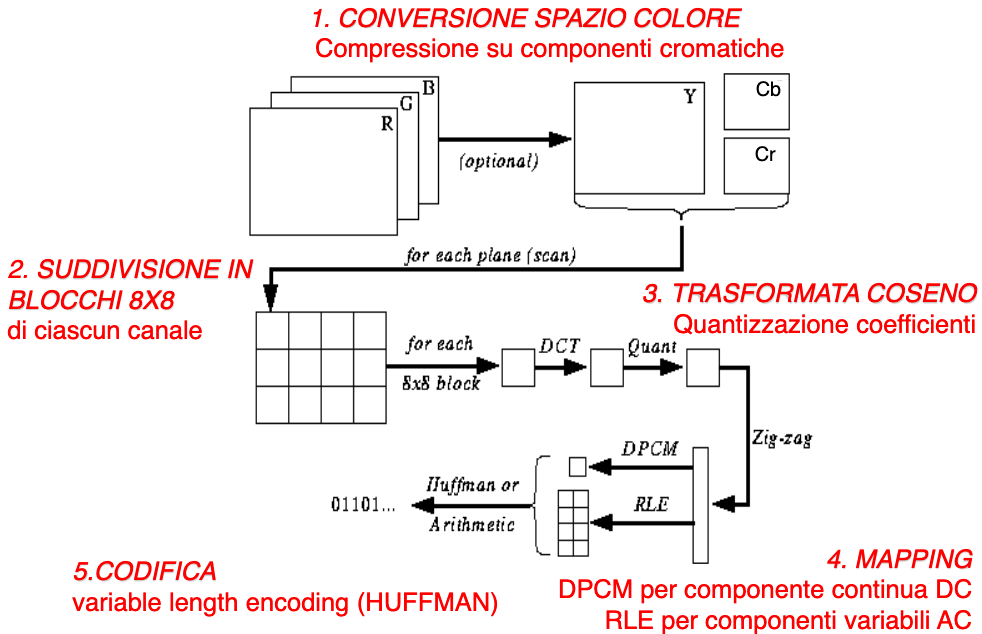
\includegraphics[scale=0.44]{Lezioni/Immagini/jpeg}
\end{figure}

La compressione JPEG si articola in 5 fasi:
\begin{enumerate}
	\item Conversione spazio colore, comprimendo le parti cromatiche;
	\item Suddivisione in blocchi 8$\times$8;
	\item Trasformata coseno e quantizzazione coefficienti;
	\item Mapping con DCPM e RLE;
	\item Codifica con Huffman.
\end{enumerate}
La perdita avviene nelle fasi di sottocampionamento del chroma e quantizzazione. 

\subsection{Conversione spazio cromatico}
Si può sfruttare la caratteristica psicovisuale per cui il sistema visivo umano è più sensibile alle variazioni di luminanza che non a quelle di crominanza, quantizzando maggiormente queste ultime.

In questo modo, la ridondanza psicovisuale diminuisce, con poca perdita. L'immagine viene convertita da RGB a un altro spazio come YCbCR, esprimendo il colore in termini di $x : y : z$ e campionando orizzontalmente.

La compressione lossy sulle coordinate cromatiche è opzionalmente effettuata riducendo le dimensioni sottocampionando tramite media a due a due tra i pixel adiacenti. 

\subsection{Suddivisione in blocchi}
Ciascun canale (Y, Cb, Cr) dell'immagine è diviso in blocchi quadrati, di cui ciascuno è costituito da 8$\times$8 pixel. 

\subsection{Analisi in frequenza}
L'idea per la quantizzazione si basa sull'utilizzo di una matrice dei coefficienti che genera coefficienti quantizzati. Le frequenze vengono pesate diversamente tagliando le alte frequenze, quindi dividendo con valori più alti, e salvando le basse applicando valori bassi.

In JPEG viene utilizzata la DCT, e i coefficienti rappresentano le ampiezze dei segnali armonici che sommati ricostruiscono il segnale.
$$F(u, v) = \sum_{x=0}^{M-1}\sum_{y=0}^{N-1} f(x, y) g(u, v, x, y)$$
$$f(x, y) = \sum_{u=0}^{M-1}\sum_{x=0}^{N-1} F(u, v) \cos\bigg[\frac{(2x + 1)\pi u}{2N}\bigg] \cos\bigg[\frac{(2x + 1)\pi v}{2N}\bigg]$$
$$g(x, y, u, v) = \alpha(u) \alpha(v) \cos\bigg[\frac{(2x + 1)\pi u}{2N}\bigg] \cos\bigg[\frac{(2y + 1)\pi v}{2N}\bigg]$$

Per ogni canale, a ogni blocco nello spazio corrisponde un blocco di coefficienti nel dominio della frequenza, in cui le basse frequenze sono in alto a sinistra e le alte sono in basso a destra. Il primo coefficiente del blocco trasformato è correlato al valore medio dei valori del blocco originario.

Viene poi definita una tabella di quantizzazione $Q$ che divide la matrice dei coefficienti $F$ e genera coefficienti quantizzati:
$$\hat{F}(u, v) = \text{round} \bigg(\frac{F(u, v)}{Q(u, v)}\bigg)$$
Le tabelle $Q(u, v)$ sono calcolate tramite esperimenti psicovisuali, scegliendo numeri che permettono una minore complessità computazionale. 

Poiché i valori della tabella di quantizzazione sono abbastanza elevati, i coefficienti quantizzati sono più piccoli e con una varianza minore. Si può variare il rapporto di compressione riscalando la tabella di quantizzazione (quality factor), che vengono poi moltiplicati in fase di decodifica:
$$ \tilde{F}(u, v) = \hat{F}(u, v) Q(u, v)$$
I coefficienti quantizzati sono ottenuti arrotondando all'intero più vicino, e quelli meno significativi tendono ad azzerarsi. 

Nelle regioni disomogenee (texture), i valori adiacenti sono distinti fra loro, e i coefficienti della matrice saranno in quantità maggiore e molto distanti dallo zero. A parità di coefficienti, la perdita è più elevata. La qualità, in generale, è buona con 16 coefficienti diversi da zero.

\subsection{Mapping dei coefficienti}
Il tipo di mapping impiegato si differenzia per i coefficienti supersititi, che possiedono una componente continua, indicata come DC, e alcune variabili, AC. Queste ultime vengono ordinate tramite zig-zag scan e codificati con RLE.

Sul valore DC invece viene applicata una tecnica DCPM (Differential Pulse Code Modulation), che codifica ogni blocco come differenza rispetto al valore del blocco precedente, sfruttando la correlazione statistica.
$$\delta_k = DC(0, 0)_k - DC(0, 0)_{k-1}$$

\subsection{Codifica dei dati}
L'ultima codifica applicata ai dati utilizza VLE (lunghezza variabile) in base all'entropia. Viene analizzata la frequenza statistica di ciascuna parola e a ognuna è assegnata una stringa del codice. 
$$p_r(r_k) = \frac{n_k}{n} \qquad L_{avg} = \sum_{k=0}^{L-1} l(r_k)p_r(r_k)$$

\begin{itemize}
	\item Codifica sequenziale: i blocchi DCT sono codificati e tramessi uno dopo l'altro, alternando le diverse componenti a colori (pagine web);
	\item Codifica progressiva: vengono trasmesse prima le porzioni più significative, visualizzando un'anteprima con qualità ridotta.
\end{itemize}

Per misurare la qualità della compressione, si usa il rapporto di compressione $C = \frac{bit_1}{bit_2}$ oppure il numero di bit per pixel. Questi valori sono dipendenti dal fattore di qualità. 

\subsection{JPEG-20}
La compressione con bit-stream ha una bassa complessità ed è efficiente, ma non esistono regioni di interesse e non è possibile differenziare la qualità.

JPEG-20 permette diverse risoluzioni, evitando i blocking artifact sfruttando una decomposizione wavelet a 3 livelli. A parità di fattore di compressione, l'immagine appare con meno blocchetti, quindi migliore.

Le zone più importanti, o meno uniformi, possono essere prioritizzate in termini di qualità, applicando una maggior compressione sullo sfondo.




%\newpage
\section{Inversioni}

\subsection{Il problema}

Come si misura la somiglianza o differenza di gusti? \\
Un esempio banale è il seguente:
\begin{gather*}
    L_A = \{1, 2, 3, 4, 5\}\\
    L_B = \{2, 4, 1, 3, 5\}
\end{gather*} \\
$L_A, L_B$ rappresentano due liste di film ordinati(con gli stessi numeri) e numerati secondo le preferenze rispettivamente di $A$ e $B$. \\
La differenza deve essere $0$ se $L_B = L_A$, e crescere fino ad avere il valore massimo quando $L_B$ è completamente "rovesciata" rispetto ad $L_A$.

\subsection{Il modello}

Una misura naturale è \textbf{il numero di inversioni(o scambi) tra film che devo fare per ricostruire } $L_A$ \textbf{ da } $L_B$ \\
Più in generale, si può arrivare alla seguente definizione:

\begin{definition}[Inversione]
    Data una sequenza di numeri $a_1,a_2,\dots,a_n$, una inversione è una coppia di indici $i < j$ tale che $a_i > a_j$.
\end{definition} ~\\
Questa definizione ci dice praticamente quanti scambi bisogna effettuare affinché l'array risulti ordinato.
$$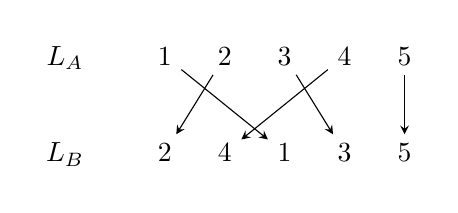
\begin{tikzpicture}
    \matrix (m) [matrix of math nodes, row sep=2em,
      column sep=1em]{
      L_A & & 1 & 2 & 3 & 4 & 5 \\
      L_B & & 2 & 4 & 1 & 3 & 5 \\};
    \path[-stealth]
        (m-1-3) edge (m-2-5)
        (m-1-4) edge (m-2-3)
        (m-1-5) edge (m-2-6)
        (m-1-6) edge (m-2-4)
        (m-1-7) edge (m-2-7);
\end{tikzpicture}$$

\subsection{Soluzioni}
~
\begin{algorithm}
    \caption{Iterativo}
    \label{inv_it}
    \begin{algorithmic}
        \Function{inverse\_count\_iterative}{$L, n$}
        \State $inv\_count \gets 0$
        \For{$i \gets 0$ \textbf{to} $n$ \textbf{step} $1$}
            \For{$j \gets 0$ \textbf{to} $i + 1$ \textbf{step} $1$}
            \State $inv\_count \gets inv\_count + 1$
            \EndFor
        \EndFor
        \EndFunction
    \end{algorithmic}
\end{algorithm}

Per ogni elemento, si conta quanti elementi alla sua destra sono più piccoli di esso.
\begin{algorithm}
    \caption{Enhanced Merge Sort}
    \label{inv_me}
    \begin{algorithmic}
        \Function{sort\_count}{$L, n$}
            \State $inv\_count \gets 0$
        \EndFunction
    \end{algorithmic}
\end{algorithm}

\newpage
\section{Problema della catena di montaggio}
In una fabbrica di automobili ci sono due catene di montaggio, ciascuna con $n$ stazioni. Due stazioni nella stessa posizione effettuano la stessa operazione ma con tempi differenti, e anche i tempi di entrata e uscita dalle catene possono essere diversi. Il passaggio tra una stazione e un'altra comporta un tempo variabile. \par

Ogni scelta delle stazioni determina univocamente un percorso. Il problema è individuare il percorso che richiede il minimo tempo totale. \\
Calcolare tutte le soluzioni possibili sarebbe computazionalmente impossibile, in quanto richiede un tempo di $2^n$. \par 

Una soluzione ottima si ottiene combinando soluzioni ottime di sotto-problemi. Siano $S_{k_1,\:1},\:S_{k_2,\:2},\:\dots \:,\:S_{k_n,\:n}$ le stazioni relative a una soluzione ottima, con $k_j\:=\:0$ oppure $k_j\:=\:1$. Per ogni $j\:=1,\: \dots, \:n$ la sequenza $S_{k_1,\:1},\:S_{k_2,\:2},\:\dots \:,\:S_{k_j,\:j}$ è la via più breve per arrivare alla stazione $S_{k_j,\:j}$. \par 
Il prossimo passo è esprimere ricorsivamente la soluzione ottima in termine di soluzione di sotto-problemi. 

%\section{Fibonacci-Strassen}

\subsection{Prodotto di matrici $n \times n$}

Esistono due soluzioni a questo problema.
\begin{enumerate}
    \item Algoritmo immediato \begin{enumerate}
        \item $O(n^3)$ somme prodotti/reali
    \end{enumerate}
    \item Algoritmo di Strassen(1969) \begin{enumerate}
        \item Per $n = 1$: $1$ prodotto e $0$ somme di reali
        \item Per $n = 2$: $7$ moltiplicazioni e $18$ addizioni(sarebbero $8$ e $4$ con l'algoritmo immediato)
    \end{enumerate}
\end{enumerate}

\begin{gather}
A = \begin{pmatrix}
    a_{1,1} & a_{1,2} \\
    a_{2,1} & a_{2,2}
\end{pmatrix} B = \begin{pmatrix}
    b_{1,1} & b_{1,2} \\
    b_{2,1} & b_{2,2}
\end{pmatrix} \\
C = A \cdot B = \begin{pmatrix}
    c_{1,1} & c_{1,2} \\
    c_{2,1} & c_{2,2}
\end{pmatrix}
\end{gather}

\subsection{La soluzione}

L'\textbf{Algoritmo di Strassen} applica i seguenti calcoli per ottenre la matrice finale $C$:
Moltiplicazioni:
\begin{gather}
    P_1 = (a_{1,1} + a_{2,2})\cdot(b_{1,1} + b_{2,2} \\
    P_2 = (a_{2,1} + a_{2,2}) \cdot b_{1,1} \\
    P_3 = a_{1,1} \cdot (b_{1,2} - b_{2,2}) \\
    P_4 = a_{2,2} \cdot (b_{2,1} - b_{1,1}) \\
    P_5 = (a_{1,1} + a_{1,2}) \cdot b_{2,2} \\
    P_6 = (a_{2,1} - a_{1,1}) \cdot (b_{1,1} + b_{1,2}) \\
    P_7 = (a_{1,2} - a_{2,2}) \cdot (b_{2,1} + b_{2,2})
\end{gather}
Somme:
\begin{gather}
    C_{1,1} = P_1+P_4-P_5+P_7 \\
    C_{1,2} = P_3 + P_5 \\
    C_{2,1} = P_2 + P_4 \\
    C_{2,2} = P_1 + P_3 - P_2 + P_6
\end{gather}
Per $n = 2^{k+1}$: riducibile a $7$ moltiplicazioni e $18$ somme di matrici di ordine $2^k$. \\
Numero di operazioni: \begin{enumerate}
    \item Prodotti: \begin{enumerate}
        \item $P(1) = 1$ 
        \item $P(2^{k+1}) = 7 \cdot P(2^k)$
    \end{enumerate}
    \item Somme: \begin{enumerate}
        \item $S(1) = 0$
        \item $S(2^{k+1}) = 7 \cdot S(2^k) + 18 \cdot 2^{2k}$
    \end{enumerate}
\end{enumerate}

\end{document}